%-  LaTeX source file

%-  main.tex ~~
%
%   This is the "main" document file, which means it is the one that will
%   \include all the other source files.
%
%                                                       ~~ (c) SRW, 20 Sep 2018
%                                                   ~~ last updated 23 Sep 2018

%%%%%%%%%%%%%%%%%%%%%%%%%%%%%%%%%%%%%%%%%%%%%%%%%%%%%%%%%%%%%%%%%%%
%
% This is a general template file for the LaTeX package SVJour3
% for Springer journals.          Springer Heidelberg 2010/09/16
%
% Copy it to a new file with a new name and use it as the basis
% for your article. Delete % signs as needed.
%
% This template includes a few options for different layouts and
% content for various journals. Please consult a previous issue of
% your journal as needed.
%
%%%%%%%%%%%%%%%%%%%%%%%%%%%%%%%%%%%%%%%%%%%%%%%%%%%%%%%%%%%%%%%%%%%
%
% First comes an example EPS file -- just ignore it and
% proceed on the \documentclass line
% your LaTeX will extract the file if required
\begin{filecontents*}{images/example.eps}
%!PS-Adobe-3.0 EPSF-3.0
%%BoundingBox: 19 19 221 221
%%CreationDate: Mon Sep 29 1997
%%Creator: programmed by hand (JK)
%%EndComments
gsave
newpath
  20 20 moveto
  20 220 lineto
  220 220 lineto
  220 20 lineto
closepath
2 setlinewidth
gsave
  .4 setgray fill
grestore
stroke
grestore
\end{filecontents*}
%
\RequirePackage{fix-cm}
%
%\documentclass{svjour3}                     % onecolumn (standard format)
%\documentclass[smallcondensed]{svjour3}     % onecolumn (ditto)
\documentclass[smallextended]{svjour3}       % onecolumn (second format)
%\documentclass[twocolumn]{svjour3}          % twocolumn

\smartqed  % flush right qed marks, e.g. at end of proof

\usepackage{graphicx}
\usepackage{amsmath}
\usepackage{hyperref}
\usepackage{listings}
\usepackage{algorithm}
\usepackage[noend]{algpseudocode}

\begin{document}

\title{Production Workload Management on Leadership Class Facilities\thanks{Grants or other notes about the article that should go on the front page should be
placed here. General acknowledgments should be placed at the end of the article.}
}
\subtitle{Do you have a subtitle?\\ If so, write it here}

%\titlerunning{Short form of title}        % if too long for running head

\author{First Author         \and
        Second Author %etc.
}

%\authorrunning{Short form of author list} % if too long for running head

\institute{F. Author \at
              first address \\
              Tel.: +123-45-678910\\
              Fax: +123-45-678910\\
              \email{fauthor@example.com}           %  \\
%             \emph{Present address:} of F. Author  %  if needed
           \and
           S. Author \at
              second address
}

\date{Received: date / Accepted: date}
% The correct dates will be entered by the editor

\maketitle

% ---------------------------------------------------------------------------
% ABSTRACT
% ---------------------------------------------------------------------------

\begin{abstract}
Insert your abstract here. Include keywords, PACS and mathematical
subject classification numbers as needed.
\keywords{First keyword \and Second keyword \and More}
% \PACS{PACS code1 \and PACS code2 \and more}
% \subclass{MSC code1 \and MSC code2 \and more}
\end{abstract}


% ---------------------------------------------------------------------------
% I - INTRODUCTION
% ---------------------------------------------------------------------------

\section{Introduction}
\label{sec:intro}
%-  LaTeX source file

%-  introduction.tex ~~
%                                                   ~~ last updated 24 Sep 2018

Traditionally, the ATLAS experiment at LHC has utilized distributed resources
as provided by the WLCG to support data distribution and enable the simulation
of events.  For example, the ATLAS experiment uses a geographically distributed
grid of approximately 200,000 cores continuously (250,000 cores at peak), (over
1,000 million core-hours per year) to process, simulate, and analyze its data
(today's total data volume of ATLAS is more than 300 PB). After the early
success in discovering a new particle consistent with the long awaited Higgs
boson, ATLAS is starting the precision measurements necessary for further
discoveries that will become possible by much higher LHC collision energy and
rates from Run2. The need for simulation and analysis will overwhelm the
expected capacity of WLCG computing facilities unless the range and precision
of physics studies will be curtailed.

Over the past few years, the ATLAS experiment has been investigating the
implications of using high-performance computers -- such as those found at Oak
Ridge leadership class facility (ORNL). This steady transition is a consequence
of application requirements (e.g., greater than expected data production),
technology trends and software complexity.

Our approach to the exascale involve the BigPanDA workload management system
which is responsible for coordination of tasks, orchestration of resources and
job submission and management. Historically, BigPanDA was used to for workload
management across multiple distributed resources on the WLCG. We describe the
changes to the BigPanDA software system needed to enable BigPanDA to utilize
Titan. We will then describe how architectural, algorithmic and software
changes have also been addressed by ATLAS computing.

We quantify the impact of this sustained and steady uptake of supercomputers
via BigPanDA: For the latest 18 month period for which data is available, Big
Panda has enabled the utilization of $\sim$400 Million Titan core
hours (primarily via Backfill mechanisms 275M, but also through regular ``front
end'' submission as part of the ALCC project 125M). This non-trivial amount of
400 million Titan core hours has resulted in 920 million events being analysed.
Approximately 3-5\% of all of ATLAS compute resources now provided by Titan;
other DOE supercomputers provide non-trivial compute allocations. In spite of
these impressive numbers, there is a need to further improve the uptake and
utilization of supercomputing resources to improve the ATLAS prospects for Run
3. 

In spite of these impressive numbers, there is a need to further improve the
uptake and utilization of supercomputing resources to improve the ATLAS
prospects for Run 3. The aim of this paper to (i) \ldots (ii) \ldots (iiii)
\ldots (iv) We will outline how we have steadily made the ATLAS project ready
for the exascale era \ldots 

%-  vim:set syntax=tex:


% ---------------------------------------------------------------------------
% II - PanDA Workload Management System: Software System Overview
% ---------------------------------------------------------------------------

\section{PanDA Workload Management System: Software System Overview}
\label{sec:overview}
PanDA is a Workload Management System (WMS)~\cite{marco2009glite} designed to
support the execution of workloads in GRID-like distributed computing
environment  via pilots~\cite{turilli2017comprehensive}.  Pilot-capable WMS
enable high throughput of tasks execution via multi-level scheduling while
supporting interoperability across multiple sites. This is particularly
relevant for LHC experiments, where millions of tasks are executed across
multiple sites of the LHC Computing Grid (LCG) every month, analyzing and
producing petabytes of data. The design of PanDA WMS started in 2005 to
support ATLAS.

% ---------------------------------------------------------------------------
\subsection{Design}
\label{subsec:design}

PanDA's application model assumes tasks grouped into workloads. Tasks
represent a set of homogeneous operations performed on datasets stored in a
set of input files. Tasks are decomposed into jobs, where each job consists
of the task's operations performed on a partition of the task's data set.
PanDA acts as an unified interface to distributed computing resources,
enabling users of the ATLAS project to submit datasets for processing. One or
more task is created for each dataset and each task is partitioned into jobs
that, in turn, are distributed across the available resources for concurrent
execution. So called ``production'' workflows are sets of transformations of
collected and simulated data into formats which are required for user
analysis.

PanDA's security model is based on separation among authentication,
authorization and accounting for both single users and group of users. Both
authentication and authorization are based on digital certificates and on the
virtual organization abstraction~\cite{foster2001anatomy}. Currently, PanDA's
execution model is based on four main abstractions: task, job, global queue,
and pilot. Both tasks and jobs are assumed to have attributes and states and
to be queued into a global queue for execution. Prioritization and binding of
jobs are assumed to depend on the attributes of each task and  job. PanDA has
a global queue where all jobs are registered and one resource queue for each
target  computing resource. PanDA assigns specific sets of jobs from the
global queue to the resource queues, depending on the jobs requirements, and
each resource capability and availability. When pilots become available on
the the target compute resource, PanDA  sends jobs on each pilot from the
resource  queue associated with that target compute source.

In PanDA's data model, each datum refers to the recorded or simulated
measurement of a physical process. Data are stored in files that are grouped
into datasets, with a relation N:N between files and datasets. As with jobs,
data have both attributes and states, and some of the attributes are shared
among events and jobs. Raw, reconstruction, and simulation data are all
assumed to be distributed across multiple storage facilities and managed by
the ATLAS Distributed Data Management (DDM)~\cite{garonne2012atlas}. When
necessary, input files required by each job are assumed to be replicated over
the network, both for input and output data. PanDA's design supports
provenance and traceability for both jobs and data. Attributes enable
provenance by linking jobs and data items, providing information like
ownership or project affiliation. States enable traceability by providing
information about the stage of the execution in which each job or data file
is or has been.

% ---------------------------------------------------------------------------
\subsection{Implementation and Execution}
\label{subsec:implementation}

The implementation of PanDA WMS consists of several interconnected
subsystems, most of them built from off-the-shelf and Open Source components.
Subsystems communicate via messaging using HTTP and dedicated APIs, and each
subsystem is implemented by one or more modules. Databases are used to store
eventful entities like tasks, jobs, and input/output data and to store
information about sites, resources, logs, and accounting.

Currently, PanDA's architecture has five main subsystems:
PanDA Server \cite{maeno2011overview},
AutoPyFactory \cite{caballero2012autopyfactory]},
PanDA Pilot \cite{nilsson2011atlas},
JEDI \cite{borodin2015scaling},
and PanDA Monitoring \cite{klimentov2011atlas}. PanDA uses ATLAS Grid
Information system (AGIS) \cite{1742-6596-513-3-032001} to obtain information
about distributed resources.

Other subsystems are used by some of ATLAS workflows (e.g., ATLAS Event
Service \cite{calafiura2015atlas}), but their discussion is omitted here
because they are irrelevant to understanding how PanDA has been ported to
supercomputers. For a full list of subsystems, see Ref.~\cite{panda-wiki_url}.
Figure \ref{fig:architecture} shows a diagrammatic representation of PanDA's
main subsystems, highlighting the execution process of tasks while omitting
monitoring details to improve readability. During first LHC data taking
period (LHC Run 1), PanDA required users to perform a static conversion
between tasks and jobs; tasks were described as a set of jobs and then
submitted to the PanDA Server. This introduced inefficiency both with
usability and resource utilization. Ideally, users should conceive analyses
in terms of one or more potentially related tasks, while the workload manager
(i.e., PanDA) should partition tasks into jobs, depending on execution
constraints. Further, the static partitioning of tasks into jobs does not
take into account the heterogeneous and dynamic nature of the resources on
which each job will be executed, introducing inefficiencies.

% For two-column wide figures use
\begin{figure*}
% Use the relevant command to insert your figure file.
% For example, with the graphicx package use
  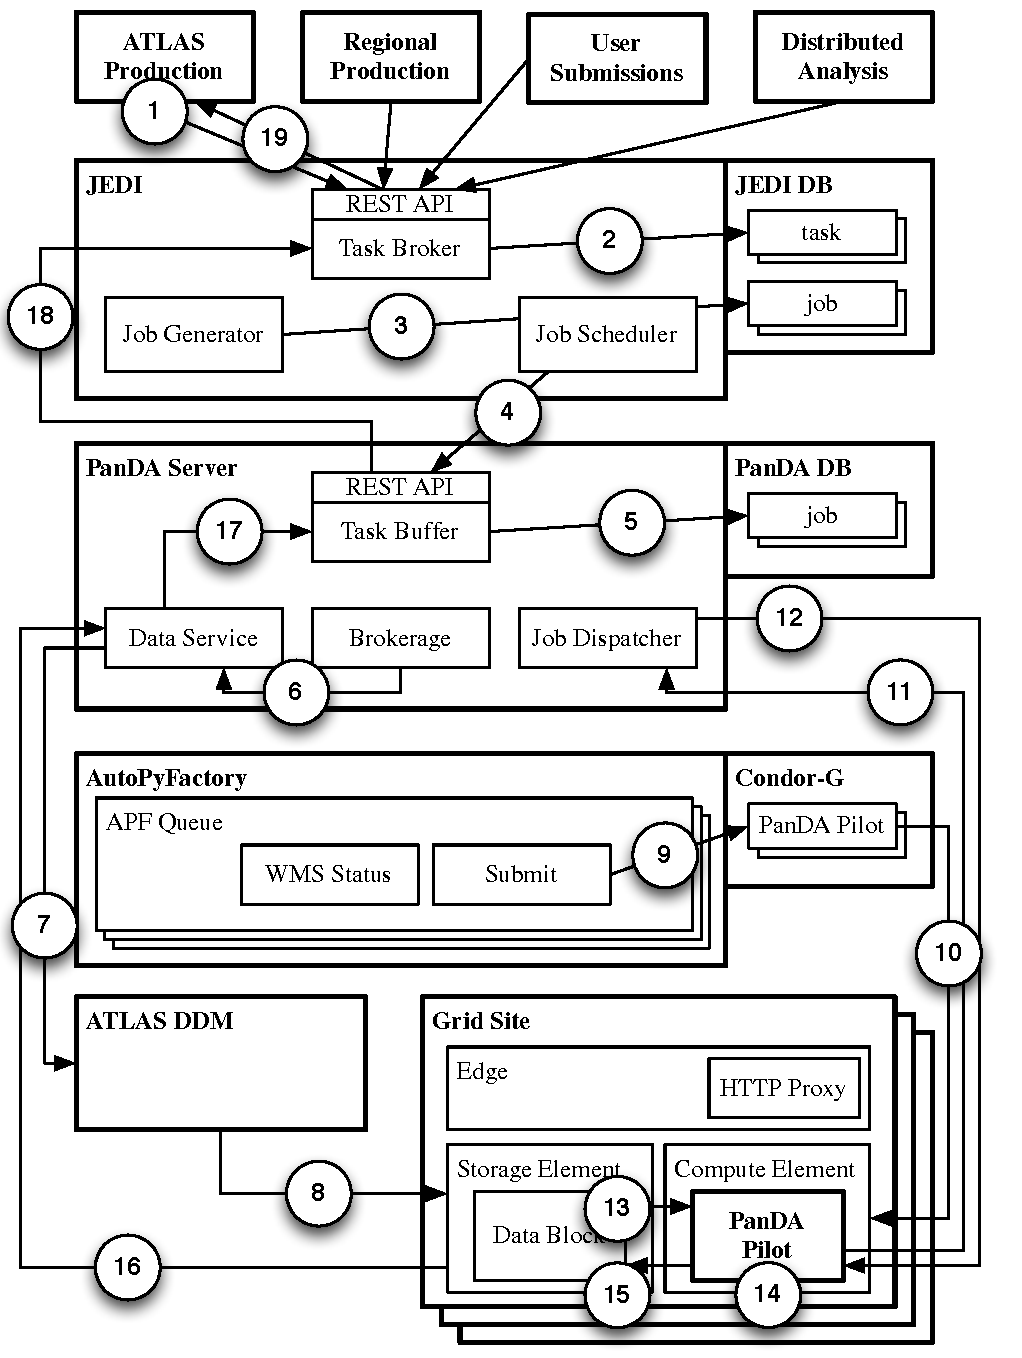
\includegraphics[width=0.75\textwidth]{images/Figure_1.pdf}
% figure caption is below the figure
\caption{PanDA WMS architecture. Numbers indicate the JEDI-based execution
process described in section \ref{subsec:implementation}. Several subsystems,
components, and architectural and communication details are abstracted to
improve clarity.}
\label{fig:architecture}
\end{figure*}

% OKAY, PROBLEM. I think the "Fig. 1:n" stuff in the next paragraph refers
% not to a new figure, but to specific numbered pieces of Figure 1. I'm going
% to link them all to the figure and hardcode the ":n" part but not the
% figure number.

Another problem of static job sizing is that PanDA instantiates pilots on
sites with different type of resources and different models of availability
of those resources. An optimal sizing of each job should take these
properties into account. For example, sites may offer cores with different
speeds, networking with different amounts of bandwidth, and resources with
different availabilities which may or may not be guaranteed for known amounts
of time. These resources could disappear at any point in time, as often
happens with opportunistic models of resource provision. JEDI system was
deployed to address these inefficiencies. Users submit task descriptions to
JEDI (Fig.~\ref{fig:architecture}:1), which stores them into a queue
implemented by a database (Fig.~\ref{fig:architecture}:2). Tasks are
partitioned into jobs of different sizes, depending on both static and
dynamic information about available resources
(Fig.~\ref{fig:architecture}:3). Jobs are bound to sites with resources that
best match jobs' requirements, and they are submitted to the PanDA Server for
execution (Fig.~\ref{fig:architecture}:4).

Once submitted to the PanDA Server, tasks are stored by the Task Buffer
component into a global queue implemented by a database
(Fig.~\ref{fig:architecture}:5). When jobs are submitted directly to the
PanDA Server, the Brokerage module is used to bind jobs to available sites,
depending on static information about the resources available for each site.
Jobs submitted by JEDI are already bound to sites, so no further brokerage is
needed.

Once jobs are bound to sites, the Brokerage module communicates to the Data
Service module about which datasets need to be made available to which sites
(Fig.~\ref{fig:architecture}:6). The Data Service communicates these
requirements to the ATLAS DDM (Fig.~\ref{fig:architecture}:7) which
replicates datasets at the required sites when needed
(Fig.~\ref{fig:architecture}:8).

Meanwhile, AutoPyFactory defines PanDA Pilots, submitting them to a Condor-G
agent (Fig.~\ref{fig:architecture}:9). Condor-G schedules these pilots
wrapped as jobs or virtual machines to the required sites
(Fig.~\ref{fig:architecture}:10).

When a PanDA Pilot becomes available, it requests a job to execute from the
Job Dispatcher module of the PanDA Server (Fig.~\ref{fig:architecture}:11).
The Job Dispatcher interrogates the Task Buffer module for a job which is
bound to the site of that pilot and ready to be executed. Task Buffer checks
the global queue (i.e., the PanDA database) and returns a job to the Job
Dispatcher if one is available. The Job Dispatcher dispatches that job to the
PanDA Pilot (Fig.~\ref{fig:architecture}:12).

Upon receiving a job, a PanDA Pilot starts a monitoring process and forks a
subprocess for the execution of the job's payload. Input data are transferred
from the stage-in location (Fig.~\ref{fig:architecture}:13) and the job's
payload is executed (Fig.~\ref{fig:architecture}:14). Once completed, output
is transferred to the staging-out location (Fig.~\ref{fig:architecture}:15).

The Data Service module of the PanDA Server tracks and collects the output
generated by each job (Fig.~\ref{fig:architecture}:16), updating jobs'
attributes via the Task Buffer module (Fig.~\ref{fig:architecture}:17). When
the output of all the jobs of a task are retrieved, it is made available to
the user via PanDA Server. When a task is submitted to JEDI, task is instead
marked as done (Fig.~\ref{fig:architecture}:18) and the result of its
execution is made available to the user by JEDI
(Fig.~\ref{fig:architecture}:19).

% ---------------------------------------------------------------------------
\subsection{Job-State Definitions in PanDA}
\label{subsec:jobstatedefs}

The lifecycle of the job in the PanDA system is splitted to the series of
consequently changing states. Each state literally coupled with the PanDA job
status used by the different algorithms and monitoring. Status reflect the
current step of the job processing since the job submitted to the system,
transferred to the particular resource and finally executed.

% For two-column wide figures use
\begin{figure*}
% Use the relevant command to insert your figure file.
% For example, with the graphicx package use
  \includegraphics[width=0.75\textwidth]{images/job-state-diagram.png}
% figure caption is below the figure
\caption{This is a job state transitions model diagram for PanDA.}
\label{fig:jobstates}
\end{figure*}

Job injected into the system by the JEDI in ATLAS or by the PanDA client in
general case is persist as so-called job parameters object and corresponds to
the ``Pending'' status. Job parameters are the object where job definition is
unsorted and all parameters are placed in a string. Sorting out parameters of
the job by dedicated DB fields job transferring into the ``Defined'' status.
On this stage the job is processed throw the brokerage algorithm and being
assigned to particular resource (PanDA queue) it is moved to ``Assigned''
status. Concurrently with that PanDA server checks availability of the input
data and needed SW at the resource. The job stays in the ``Waiting'' state
until data and the SW are ready and then it moved to the ``Activated''
status. Activated job is ready to be dispatched by its order to the next
corresponding pilot. Job dispatched and taken by the pilot is moved to the
``Sent'' status. Since this moment the handling of the job processing is
delegated to the pilot. Few next job states are corresponding represents the
steps of the job processing on the resource. Next ``Starting'' status means
that the pilot is starting the job on a worker node or local batch system.
The job running on a worker node marked as in ``Running'' status. Next states
progression is return to the handling by the server. When the job execution
is ended and output and log files are transferred then PanDA server either
pilot is responsible to register that files in the file catalog. At the same
time pilot return the server the final status of the job either it was
successful or the job failed. During this process the job stays in
``Holding'' status. PanDA server check the output files regularly by the cron
job and finally assign the final ``Finished'' or ``Failed'' status to the
job. Some additional statuses and two most important are ``Cancelled'' for
manually killed jobs or ``Closed'' - terminated by the system before
completing to be reassigned to another site.

% ---------------------------------------------------------------------------
\subsection{Brokerage Characterization}
\label{subsec:brokerage}

Resources (queues) presented in the database together with the wide set of
static parameters such as walltime, CPU cores, memory, disk space etc. Same
parameters can be provided within job definition to specify strict demands to
the resource where the job can be executed. Both resources (queues) and jobs
with parameters stored in the PanDA database.

Also PanDA server maintains in the DB the dynamic information for queues
about the number of defined, activated and running jobs and also the pilots
statistics - number of requests of different types like ``get job'' or
``update job status''.

PanDA Broker - key  component of the BigPanDA workflow automation - is an
intelligent module designed to prioritize and assign PanDA jobs (job passed
the brokerage transitioning from ``defined'' to the ``assigned'' state) to
available computing resources on the basis of job type, software
availability, input data and its locality, real-time job statistics,
available CPU and storage resources and etc. Users are able to specify
explicitly the resource while job submission or they can rely on automated
brokerage engine. Full power of the PanDA brokerage integrated with another
distributed computing and data management tools (internal and external with
respect to the PanDA) is actively used in ATLAS experiment. In this paper we
will present and will benchmark the basic brokerage functionality.

The basic brokerage algorithm works the following way. It takes the lists of
submitted jobs and available queues. Then each job is checked against each
queue by set of parameters if the queue meets the jobs static demands like
number of CPU core or the walltime. All queues passed the round are
proceeding to the short list where for each queue Broker calculates the
weight on the basis of current job statistics for given queue according to
the formula (1). Job finally assigning to the queue with bigger weight.
Weight calculation algorithm fo ATLAS is more complicated and taking into
account clouds default weights, network bandwidth, sharing policies etc.

The basic brokerage algorithm works the following way. Having the list of the
submitted jobs, each job is checked against available resources as shown in
SELECT{\textunderscore}CAND (Alg. ). Available resources presented as the set
of defined PanDA queues: res = queue$_1$, \ldots, queue$_n$. For each queue
in the set (3) we checking if it's satisfying the parameters of job (4).
Successfully passed queues are concatenating to the list of candidate-queues
(5).

SATISFY{\textunderscore}JOB function (Alg. ) is used to check if the queue
attributes can scope job parameters. Set of the job parameters defined as
par$_1$, \ldots, par$_m$ represents the software/hardware demands to the
resource like CPU core count, walltime, SW releases etc. Each of these
parameters can be mapped to the set of queue attributes defined as atr$_1$,
\ldots, atr$_n$, where $n \geq m$. So for each job parameter (2) we check if
it can be satisfied with the corresponding queue attribute (3). Finally queue
passes the test if it copes all the jobs parameters (5).

The procedure SATISFY{\textunderscore}REQ (Alg. ) is responsible to testing
if the value of the job parameter is in the set of allowed values val$_1$,
\ldots, val$_k$ of the queue attribute (2).

%-  NOTE: I think there are indenting mistakes present in the original
%   writing, because things just honestly don't look right to me, but right
%   now, I'm just typesetting what I see in Google Docs.

% I have already included the package required by this. Just put the code
% list.py file (or whatever other name you want to use.)

\lstinputlisting[language=Python, 
         label={lst:list.py}, 
         caption={Caption}]{list.py}

\begin{tabbing}
\hspace{0.5in}\=
     Require: par; atr = (val$_1$, \ldots, val$_k$) \\
  \> Ensure: True or False \\
  \> 1: \hspace{1em}\= procedure SATISFY{\textunderscore}REQ(par, atr) \\
  \> 2:             \> \hspace{1em}\= if par.value in atr then: \\
  \> 3:             \>             \> return True \\
  \> 4:             \>             \> \hspace{0.1in} return False
\end{tabbing}

\begin{tabbing}
\hspace{0.5in}\=
     Require: job = \{par$_1$, \ldots, par$_m$\}; queue = \{atr$_1$, \ldots, atr$_n$\} \\
  \> Ensure: True or False \\
  \> 1: \hspace{1em}\= procedure SATISFY{\textunderscore}JOB(queue, job) \\
  \> 2:             \> \hspace{1em}\= for all par in job do: \\
  \> 3:             \>             \> if SATISFY{\textunderscore}REQ(par, atr)%
= False then \\
  \> 4:             \>             \> \hspace{2em} return False \\
  \> 5:             \>             \> \hspace{1em} return True
\end{tabbing}

\begin{tabbing}
\hspace{0.5in}\=
     Require: job; res = (queue$_1$, \ldots, queue$_n$) \\
  \> Ensure: cand \\
  \> 1: \hspace{1em}\= procedure SELECT{\textunderscore}CAND(job, res) \\
  \> 2:             \> \hspace{1em}\= cand $\leftarrow$ NONE \\
  \> 3:             \> \hspace{1em}\= for all queue in res do: \\
  \> 4:             \>             \> if SATISFY{\textunderscore}JOB(queue, %
job) = True then \\
  \> 5:             \>             \> \hspace{1em} cand $\cup$ queue \\
  \> 6:             \>             \> return True
\end{tabbing}

As it was shown SELECT{\textunderscore}CAND procedure provides generates the
short list of the candidates queues. SELECT{\textunderscore}QUEUE (Alg. )
taking the short list of the candidate-queues as the set queue$_1$, \ldots,
queue$_n$. For each queue (4) Broker calculates the weight (5) on the basis of
current job statistics for given queue according to the formula (1). Job
finally assigning to the queue with bigger weight (6-7). Weight calculation
algorithm fo ATLAS is more complicated and taking into account clouds default
weights, network bandwidth, sharing policies etc

\begin{tabbing}
\hspace{0.5in}\=
     Require: cand = (queue$_1$, \ldots, queue$_n$) \\
  \> Ensure: res{\textunderscore}queue \\
  \> 1: \hspace{1em}\= procedure SELECT{\textunderscore}QUEUE(cand) \\
  \> 2:             \> \hspace{1em}\= res{\textunderscore}queue $\leftarrow$%
queue$_1$ \\
  \> 3:             \>             \> \hspace{0.1in} max{\textunderscore}%
weight $\leftarrow 0$ \\
  \> 4:             \> \hspace{1em}\= for all queue in cand do: \\
  \> 5:             \>             \> queue.weight $\leftarrow$ %
WEIGHT{\textunderscore}CALC(queue) \\
  \> 6:             \>             \> \hspace{1em} if queue.weight $>$ %
max{\textunderscore}weight then \\
  \> 7:             \>             \> \hspace{2em} res{\textunderscore}queue%
$\leftarrow$ queue \\
  \> 8:             \>             \> \hspace{0.5em} return %
res{\textunderscore}queue
\end{tabbing}

\begin{equation}
  \begin{aligned}
    & manyAssigned = \max(1, \min(2, \frac{assigned}{activated})), \\
    & weight = \frac{running + 1}{(activated + assigned + sharing + defined +
        10) * manyAssigned}
  \end{aligned}
\end{equation}

Response time of the brokerage in general can be estimated as (2). Basically it's time the job
transits from ``defined'' to assigned state.  

\begin{equation}
    T = \sum_{i = 1}^{Q} \sum_{j = 1}^{J} T_{ij}
\end{equation}

In formula (2) $Q$ is the number of available queues, $J$ is the number of
concurrently  submitted jobs and $T_{ij}$ is the time to process job $j$ for
queue $i$. The processing time includes the check if queue meet demands of the
job. Then for successfully selected queues the weight is calculating and job
assigning for the queue with bigger weight. Hence the time $T$ can be presented as sum (3).

\begin{equation}
T = t_1 + t_2 + t3_3 + C
\end{equation}

In formula 3, $t_1$ is the time to make checks if queue meet demands of the
job, $t_2$ is the time for weight calculation and finally $t_3$ is the time
spent to assign job to the resulted queue. 

Under the assumption that all jobs can run on the same average number of queues
$N$ then we can transform equation as (4).

\begin{equation}
T = J * \left ( \sum_{i = 1}^{Q - N} t1_j + \sum_{j = 1}^{N} (tmax + t2_j) + t3 \right) + C, t1 < tmax
\end{equation}

Here N is the average number of queues which met all demands of each job.  As shown in the SATISFY{\textunderscore}JOB algorithm the function returns FALSE as soon as the first discrepancy in the job parameter and queue attributes is met. Hence for for all other Q-N queues the time to make checks  t1 will be less than tmax.

Here N is the average number of queues which met all demands of each job. As shown in the SATISFY{\textunderscore}JOB algorithm the function returns False as
soon as the first discrepancy in the job parameter and queue attributes is met.
Hence for for all other Q-N queues the time to make checks t1 will be less than tmax.

Again taking assumption that the times for different queues are equal we can
streamline the equation like (5)

\begin{equation}
  \begin{aligned}
    T =& J * \left(( Q - N) * t1 + N * (tmax + t2) + t3 \right) + C \\
     =& J * \left(Q * t1 + N * (tmax - t1 + t2) + t3 \right) + C,
        \text{where}~(tmax - t1) > 0
  \end{aligned}
\end{equation}

In order to estimate dependency of brokerage response time from the number of
concurrently submitted jobs we deployed a dedicated test instance of PanDA
server at ORNL. PanDA was configured to use ten testing queues. Two of the
queus was configured to provide 8 CPU cores and eight remaining queues provide
2 cores. All other parameters are configured equal for all queues.

Job submission client was configured to generate and send to the server the
lists of equal jobs where each job demands 4 CPU cores. PanDA testing-instance
was adjusted to simulate the brokerage two queues will be selected as meeting
the criteria of cores number. Then due to simulation of job statistics on that
selected queues the jobs will be assigned to the queue with bigger weight.
Brokerage time dependency on number of concurrently submitted jobs is shown in
figure.

%-  The publisher prefers TIFF, and Ruslan and others have provided the images
%   in TIFF as requested. I am not aware of a LaTeX engine that understands
%   TIFF natively, and pasting shell-escape sequences from the internet is a
%   very, very bad idea, so I just converted it to PNG for now and included
%   both in the repository.

% For two-column wide figures use
\begin{figure*}
  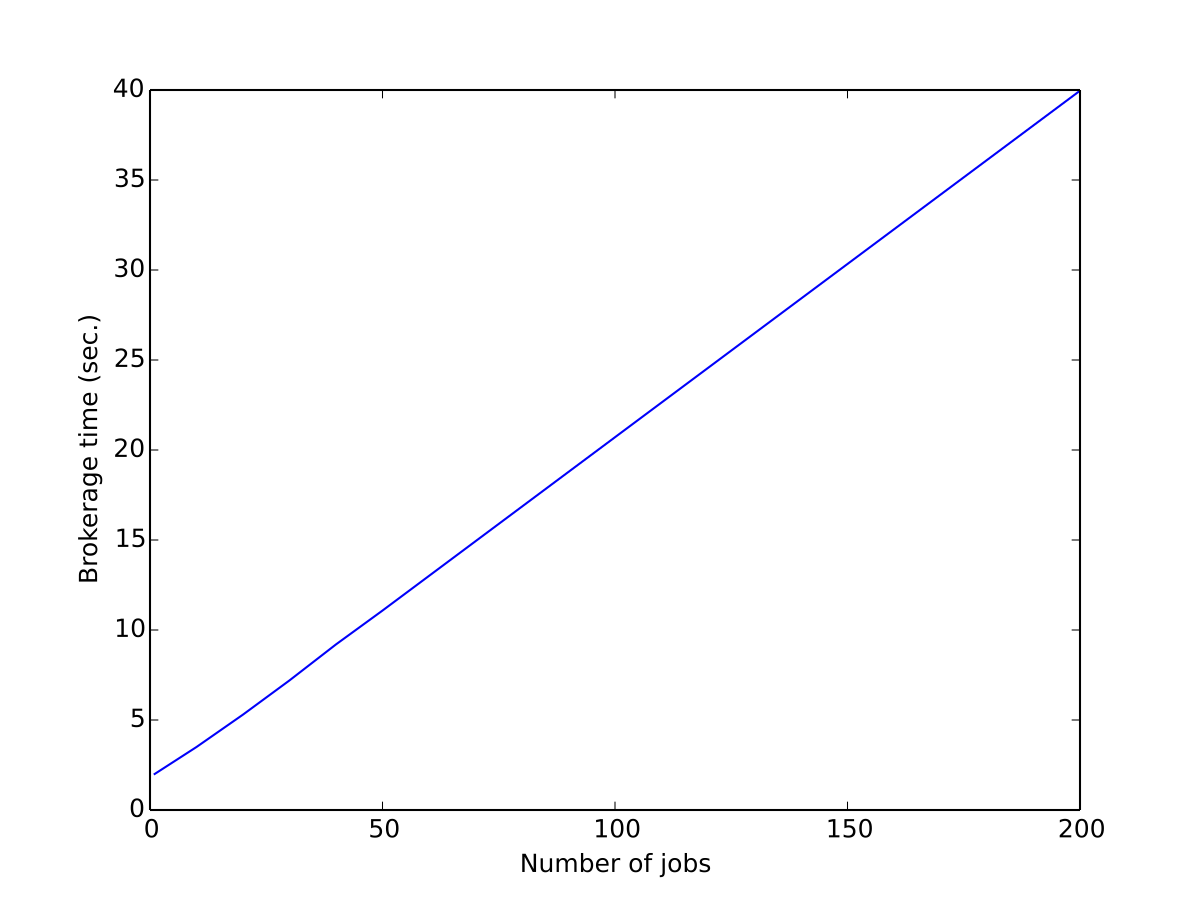
\includegraphics[width=0.75\textwidth]{images/Fig2.png}
\caption{Response time dependency on number of concurrently submitted jobs}
\label{fig:brokeragescaling}
\end{figure*}

For this experiment we measured the response time for a jobs to transit from the
``Defined'' status to the ``Activated''. As in the test environment the JEDI
system wasn't used and injection of the jobs was done using the simple python
client interaction with PanDA REST API the first stated of the job indicated in
PanDA is ``Defined'' and corresponds to the creation time. Also during this
measurements we used no-input jobs. Hence the status of the jobs progressed to
the ``Activated'' immediately after ``Defined''. In general the time to check
input files can be considered as constant for the constant number of input
files. So omitting the ``Assigned'' state in this testing environment is
acceptable. 



%-  vim:set syntax=tex:


% ---------------------------------------------------------------------------
% III - Deploying PanDA Workload Management System on Titan
% ---------------------------------------------------------------------------

\section{Deploying PanDA Workload Management System on Titan}
\label{sec:deploying}
%-  LaTeX source file

%-  deploying.tex ~~
%
%   This is the third section of the paper.
%
%                                                   ~~ last updated 24 Sep 2018

\begin{itemize}
    \item Start of project and proof of concept, restrictions caused by policy
        of usage of OLCF
    \item Adaptation of already existed PanDA application to work with Titan
    \item Many To One concept (Many jobs - one pilot)
    \item First implementation (Multijob Pilot as evolution of PanDA Pilot)
    \item Scalability limitations
    \item Harvester
\end{itemize}

Consistent with its leadership-computing mission of enabling applications of
size and complexity that cannot be readily performed using smaller facilities,
the OLCF prioritizes the scheduling of large capability jobs (or
``leadership-class'' jobs). OLCF uses batch queue policy on the Titan systems
to support the delivery of large capability-class jobs.  (Reference Titan
Scheduling Policy, \url{%
https://www.olcf.ornl.gov/for-users/system-user-guides/titan/running-jobs/})

OLCF deploys Adaptive Computing's MOAB resource manager. [Reference: Adaptive
Computing Administrator’s Guide, 6.1.2,
\url{http://docs.adaptivecomputing.com/9-1-2/MWM/Moab-9.1.2.pdf}]  MOAB
resource manager supports features that allow it to directly integrate with
Cray's Application Level Placement Scheduler (ALPS), a lower-level resource
manager unique to Cray HPC clusters. [Reference: Ezell et al., CUG 2013, \url{%
https://cug.org/proceedings/cug2013_proceedings/includes/files/pap177.pdf}].

MOAB will schedule jobs in the queue in priority order, and priority jobs will
be executed given the availability of required resources.  As a DOE Leadership
Computing Facility, the OLCF has a mandate that a large portion of Titan's
usage come from large, leadership-class (aka capability) jobs. To ensure the
OLCF user programs achieve this mission, OLCF policies strongly encourage
through queue policy users to run jobs on Titan that are as large as their
code will warrant. To that end, the OLCF implements queue policies that enable
large jobs to be scheduled and run in a timely fashion. (Ref. Titan User
Manuel, \url{%
https://www.olcf.ornl.gov/for-users/system-user-guides/titan/running-jobs/})
As a result, leadership-class jobs advance to the high-priority jobs in the
queue.

If a priority job does not fit, i.e., required resources are not available, a
resource reservation will be made for it in the future when availability can be
assured. Those nodes are exclusively reserved for that job. When the job
finishes, the reservation is destroyed, and those nodes are available for the
next job. Reservations are simply the mechanism by which a job receives
exclusive access to the resources necessary to run the job. [Reference: Ezell
et al., CUG 2013] However, if policy desires a priority reservation to be made
for more than one job, one can specify the creation of reservations for the top
N priority jobs in the queue by increasing the keyword RESERVATIONDEPTH to be
greater than one.  The priority reservation(s) will be re-evaluated (and
destroyed/re-created) every scheduling iteration in order to take advantage of
updated information.

Beyond the creation of reservations for the top priority jobs, Moab now
switches to backfill mode and continues down the job queue until it finds a job
that will be able to start and won't disturb the priority reservations made for
the highest priority queued jobs, specified by the value of RESERVATIONDEPTH.
As time continues and the scheduling algorithm continues to iterate, Moab
continues to evaluate the queue for the highest priority jobs. If the highest
priority job found will not fit within the available resources, its reservation
is updated, but left where it is. Switching to ``backfill mode'', Moab searches
for a job in the queue that will be able to start and complete without
disturbing the priority reservations.  If such jobs are started, they will run
within backfill.  If no such backfill jobs are present in the queue, then
available compute resources will remain unutilized.

In describing how the PanDA Workload management system is deployed on Titan, we
necessarily describe it integration with the Moab Workload management system.
In so doing, two rather different approaches to interfacing the PanDA managed
work on Titan are availed: ``Batch Queue Mode'' and ``Backfill Mode''.  In
``Batch Queue Mode'', PanDA interacts with Titan's Moab scheduler in a static,
non-adaptive manner to executing the work to be performed.  In ``Backfill
Mode'', PanDA  dynamically shapes the size of the work deployed on Titan to
capture resources that may otherwise go unused because the size of the backfill
opportunity is otherwise too small or to brief in duration.

In doing so, we demonstrate how Titan is more efficiently utilized by the
injection and mixing of small and short-lived tasks in backfill with regular
payloads. Cycles otherwise unusable (or very difficult to use) are used for
science, thus increasing the overall utilization on Titan without loss of
overall quality-of-service. The conventional mix of jobs at OLCF cannot be
effectively backfilled because of size, duration, and scheduling policies. Our
approach is extensible to any HPC with ``capability scheduling'' policies. 

\subsection{PanDA integration with Titan}
\label{subsec:integration}

As we described in previously PanDA is a pilot based WMS. On the Grid pilot
jobs are submitted to batch queues on compute sites and wait for the resource
to become available. When a pilot job starts on a worker node it contacts the
PanDA server to retrieve an actual payload and then, after necessary
preparations, executes the payload as a sub process. The PanDA pilot is also
responsible for a job's data management on a worker node and can perform data
stage-in and stage-out operations. Figure 3 shows schematic view of PanDA
interface.

Taking advantage of its modular and extensible design, the PanDA pilot code and
logic has been enhanced with tools and methods relevant for work on HPCs. The
pilot runs on Titan's data transfer nodes (DTNs) which allows it to communicate
with the PanDA server, since DTNs have good (10 GB/s) connectivity to the
Internet. The DTNs and the worker nodes on Titan use a shared file system which
makes it possible for the pilot to stage-in input files that are required by
the payload and stage-out produced output files at the end of the job. In other
words, the pilot acts as a site edge service for Titan. Pilots are launched by
a daemon-like script which runs in user space. The ATLAS Tier 1 computing
center at Brookhaven National Laboratory is currently used for data transfer to
and from Titan, but in principle that can be any ATLAS site. Figure 4 shows
schematic view of PanDA interface with Titan.
The pilot submits ATLAS payloads to the worker nodes using the local batch
system (Moab) via the SAGA (Simple API for Grid Applications) interface [Saga
ref needed]. It also uses SAGA for monitoring and management of PanDA jobs
running on Titan's worker nodes. One of the features of the described system is
the ability to collect and use information about Titan status, e.g., free
worker nodes in real time. The pilot can query the Moab scheduler about
currently unused nodes on Titan, using the ``showbf'' command, and check if the
free resource availability time and size are suitable for PanDA jobs, and
conforms with Titan's batch queue policies. The pilot transmits this
information to the PanDA server, and in response gets a list of jobs intended
for submission on Titan. Then based on the job information, it transfers the
necessary input data from the ATLAS Grid, and once all the necessary data is
transferred the pilot submits jobs to Titan using an MPI wrapper.

The MPI wrappers are Python scripts that are typically workload specific since
they are responsible for setup of the workload environment, organization of
per-rank worker directories, rank-specific data management, optional input
parameters modification, and cleanup on exit. When activated on worker nodes
each copy of the wrapper script after completing the necessary preparations
will start the actual payload as a subprocess and will wait until its
completion. This approach allows for flexible execution of a wide spectrum of
Grid-centric workloads on parallel computational platforms such as Titan.

Since ATLAS detector simulations are executed on Titan as discrete jobs
submitted via MPI wrapper, parallel performance can scale nearly linearly,
potentially limited only by shared file system performance (discussed below).
Currently up to 20 pilots are deployed at a time, distributed evenly over 4
DTNs. Each pilot controls from 15 to 350 ATLAS simulation ranks per submission.
This configuration is able to utilize up to 112,000 cores on Titan. We expect
that these numbers will grow in the near future.
Figure 4.4-1 shows Titan core hours consumed by the ATLAS Geant4 simulations
from January 2017 to April 2018. Please note that during this time our
Director's Discretionary project ran 24/7 in pure backfill mode with lowest
priority and no defined allocation. In 2017-2018 average resource utilization
exceeded 10M core-hours per month and for February and March of 2018 reached
22M core-hours per month. We expect that average monthly utilization will grow
due to further optimization of the workload management system.


% For two-column wide figures use
\begin{figure*}
% Use the relevant command to insert your figure file.
% For example, with the graphicx package use
  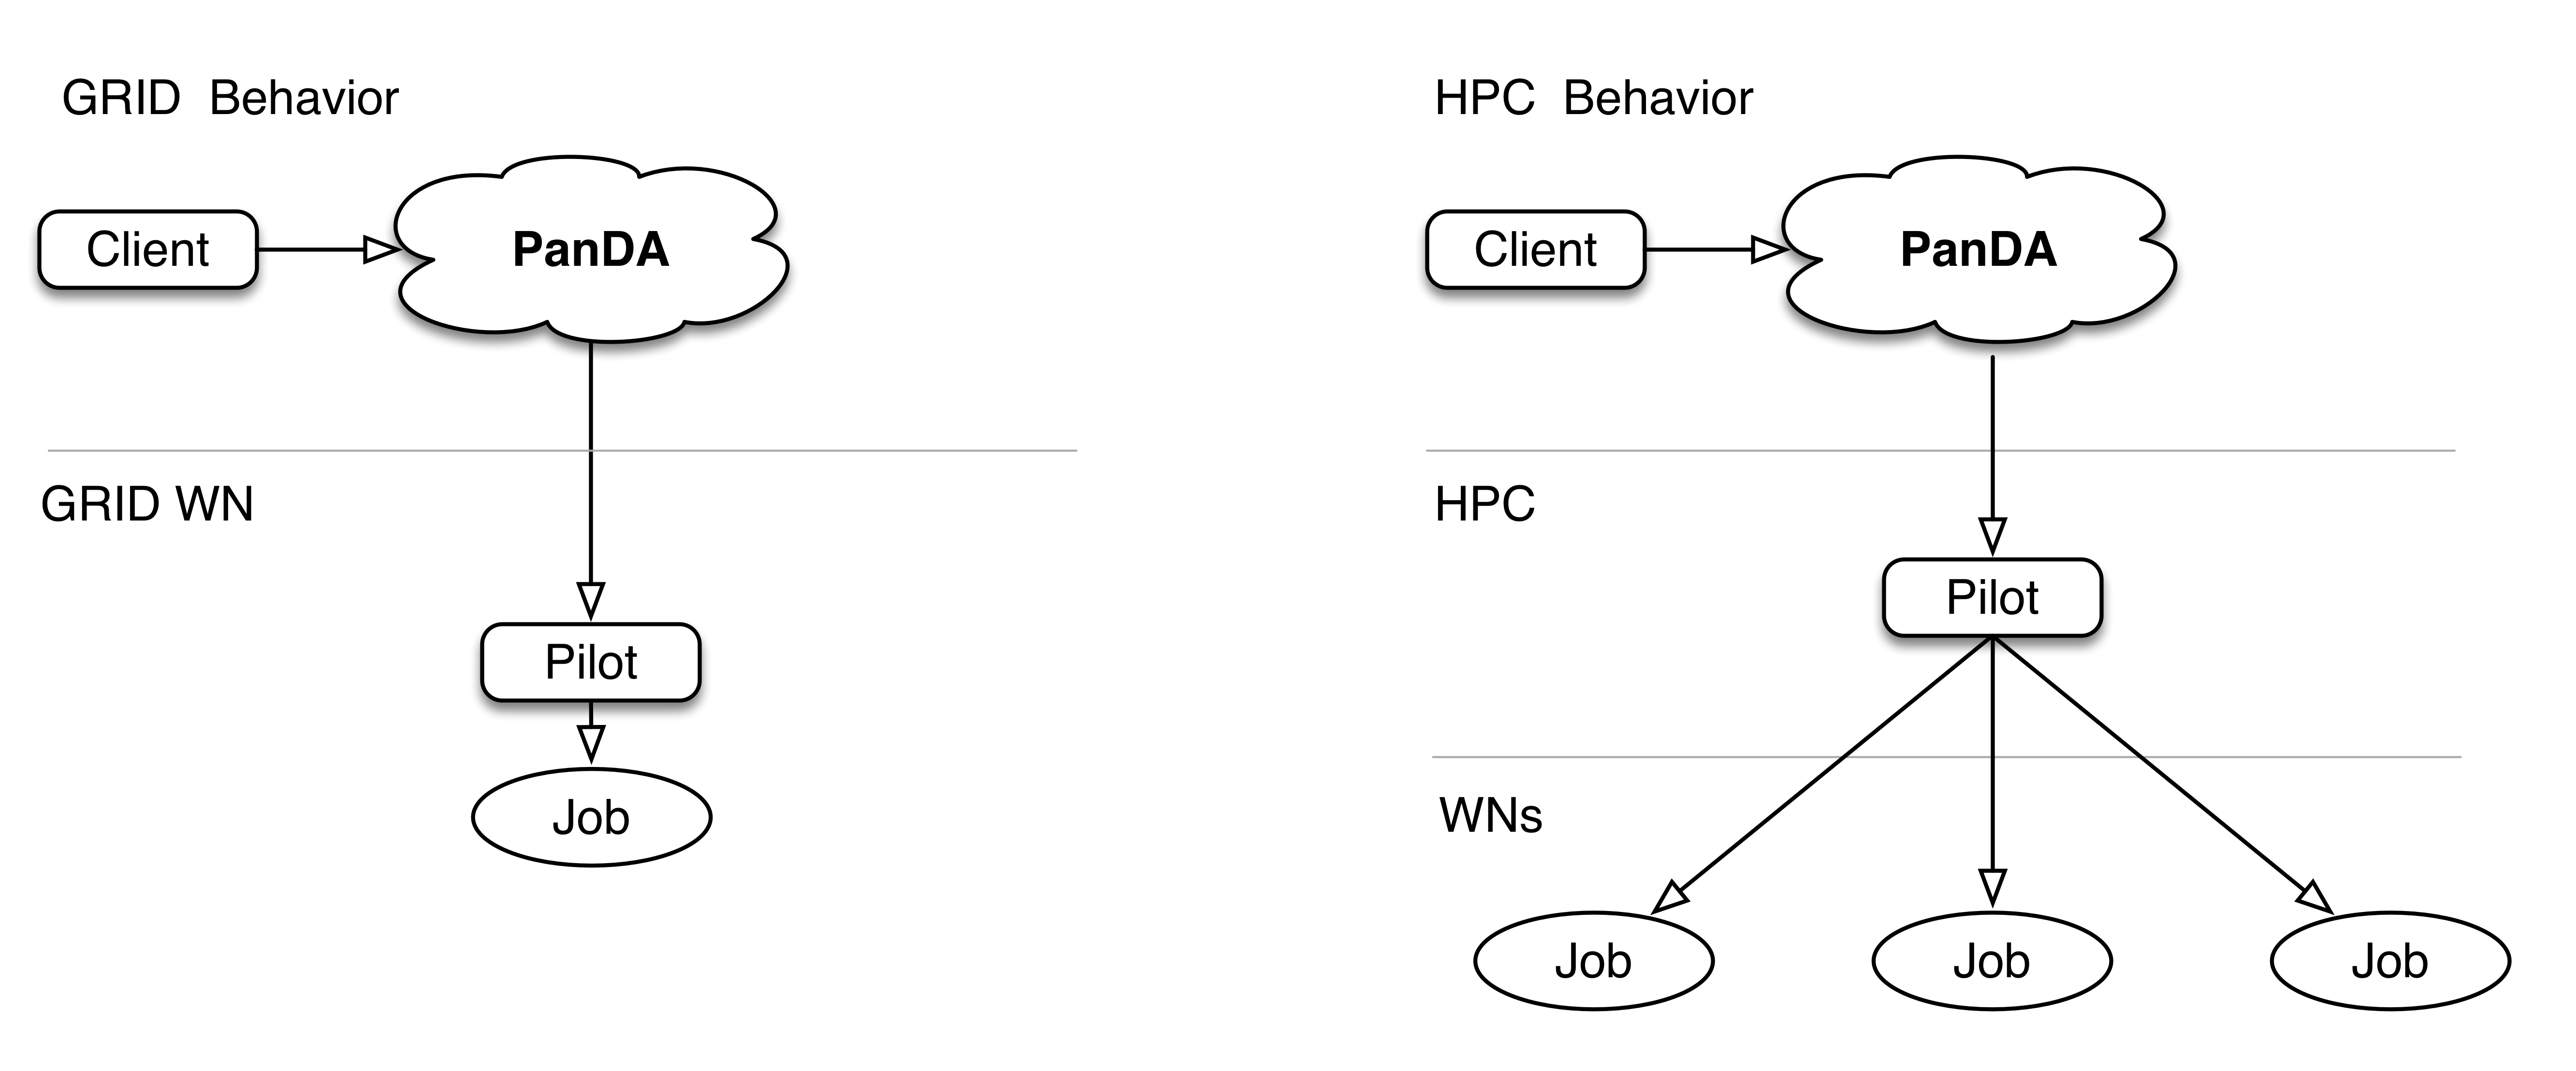
\includegraphics[width=0.75\textwidth]{images/Figure_3.png}
% figure caption is below the figure
\caption{A concept for the launching of multiple PanDA jobs on HPC with the
limited number of Job Slots in comparison with regular GRID launch}
\label{fig:launching}
\end{figure*}

% For two-column wide figures use
\begin{figure*}
% Use the relevant command to insert your figure file.
% For example, with the graphicx package use
  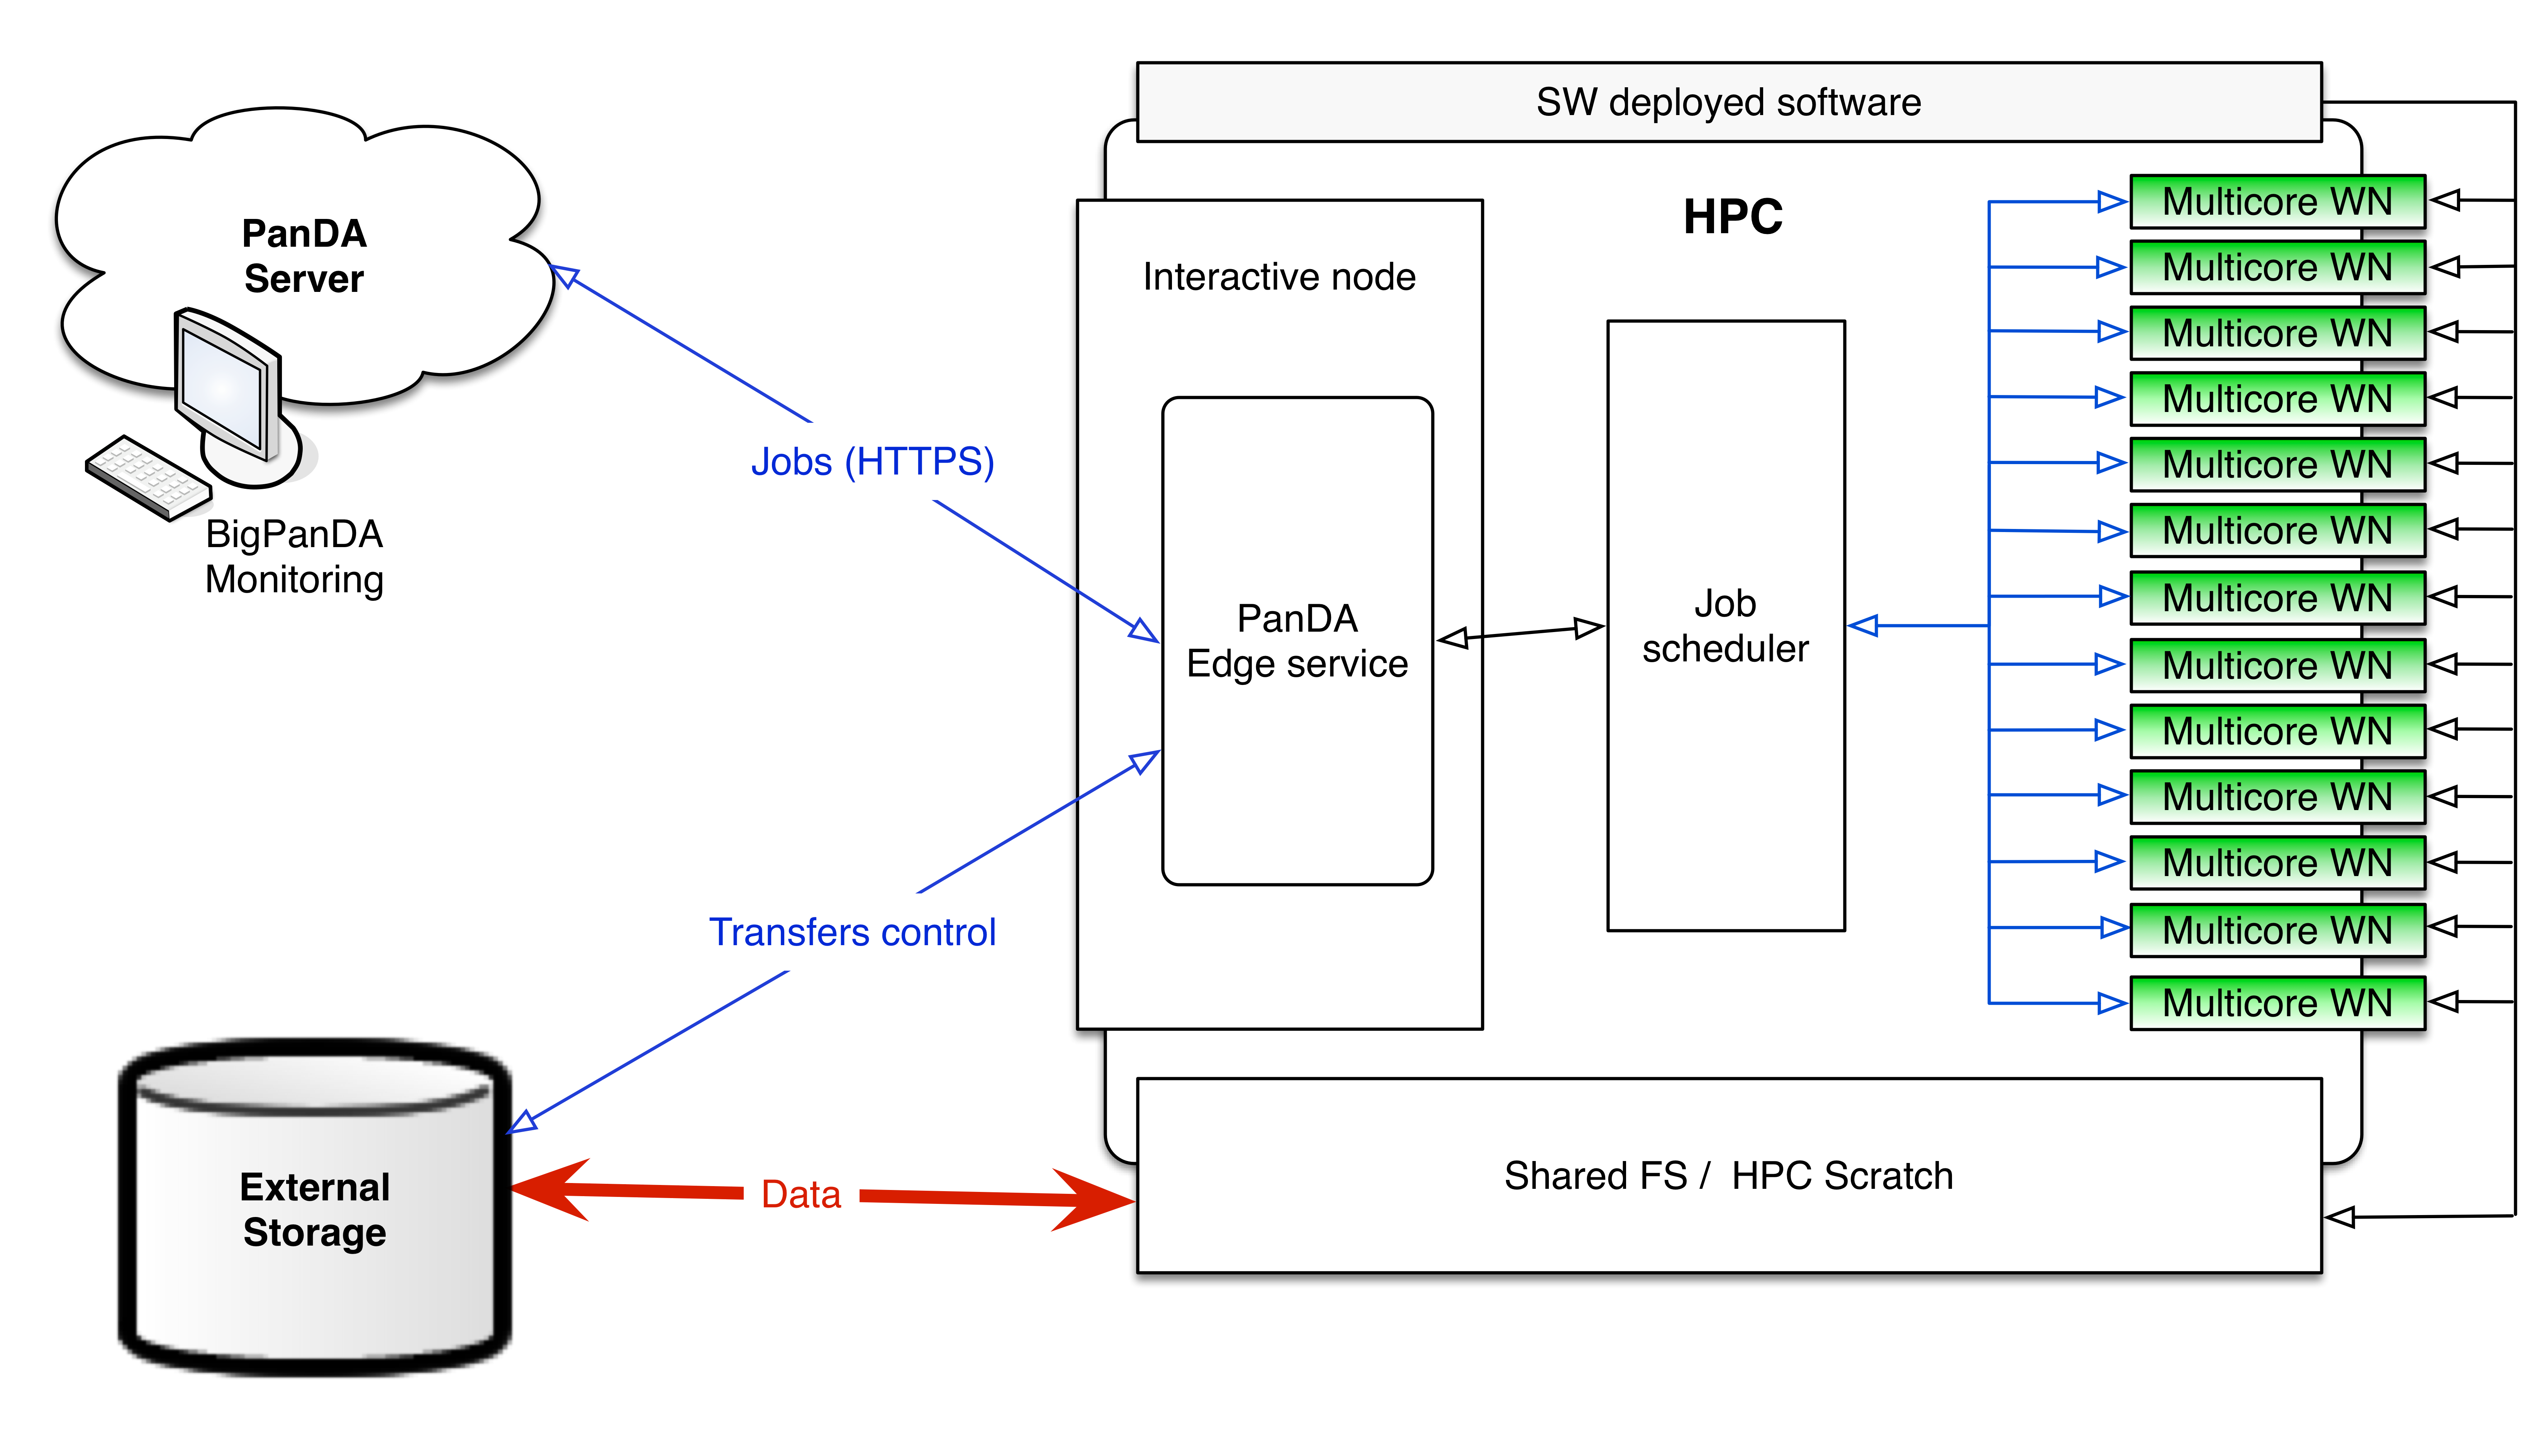
\includegraphics[width=0.75\textwidth]{images/Figure_4.png}
% figure caption is below the figure
\caption{A concept of integration of LCF(HPC) with PanDA}
\label{fig:integration}
\end{figure*}

% For two-column wide figures use
\begin{figure*}
% Use the relevant command to insert your figure file.
% For example, with the graphicx package use
  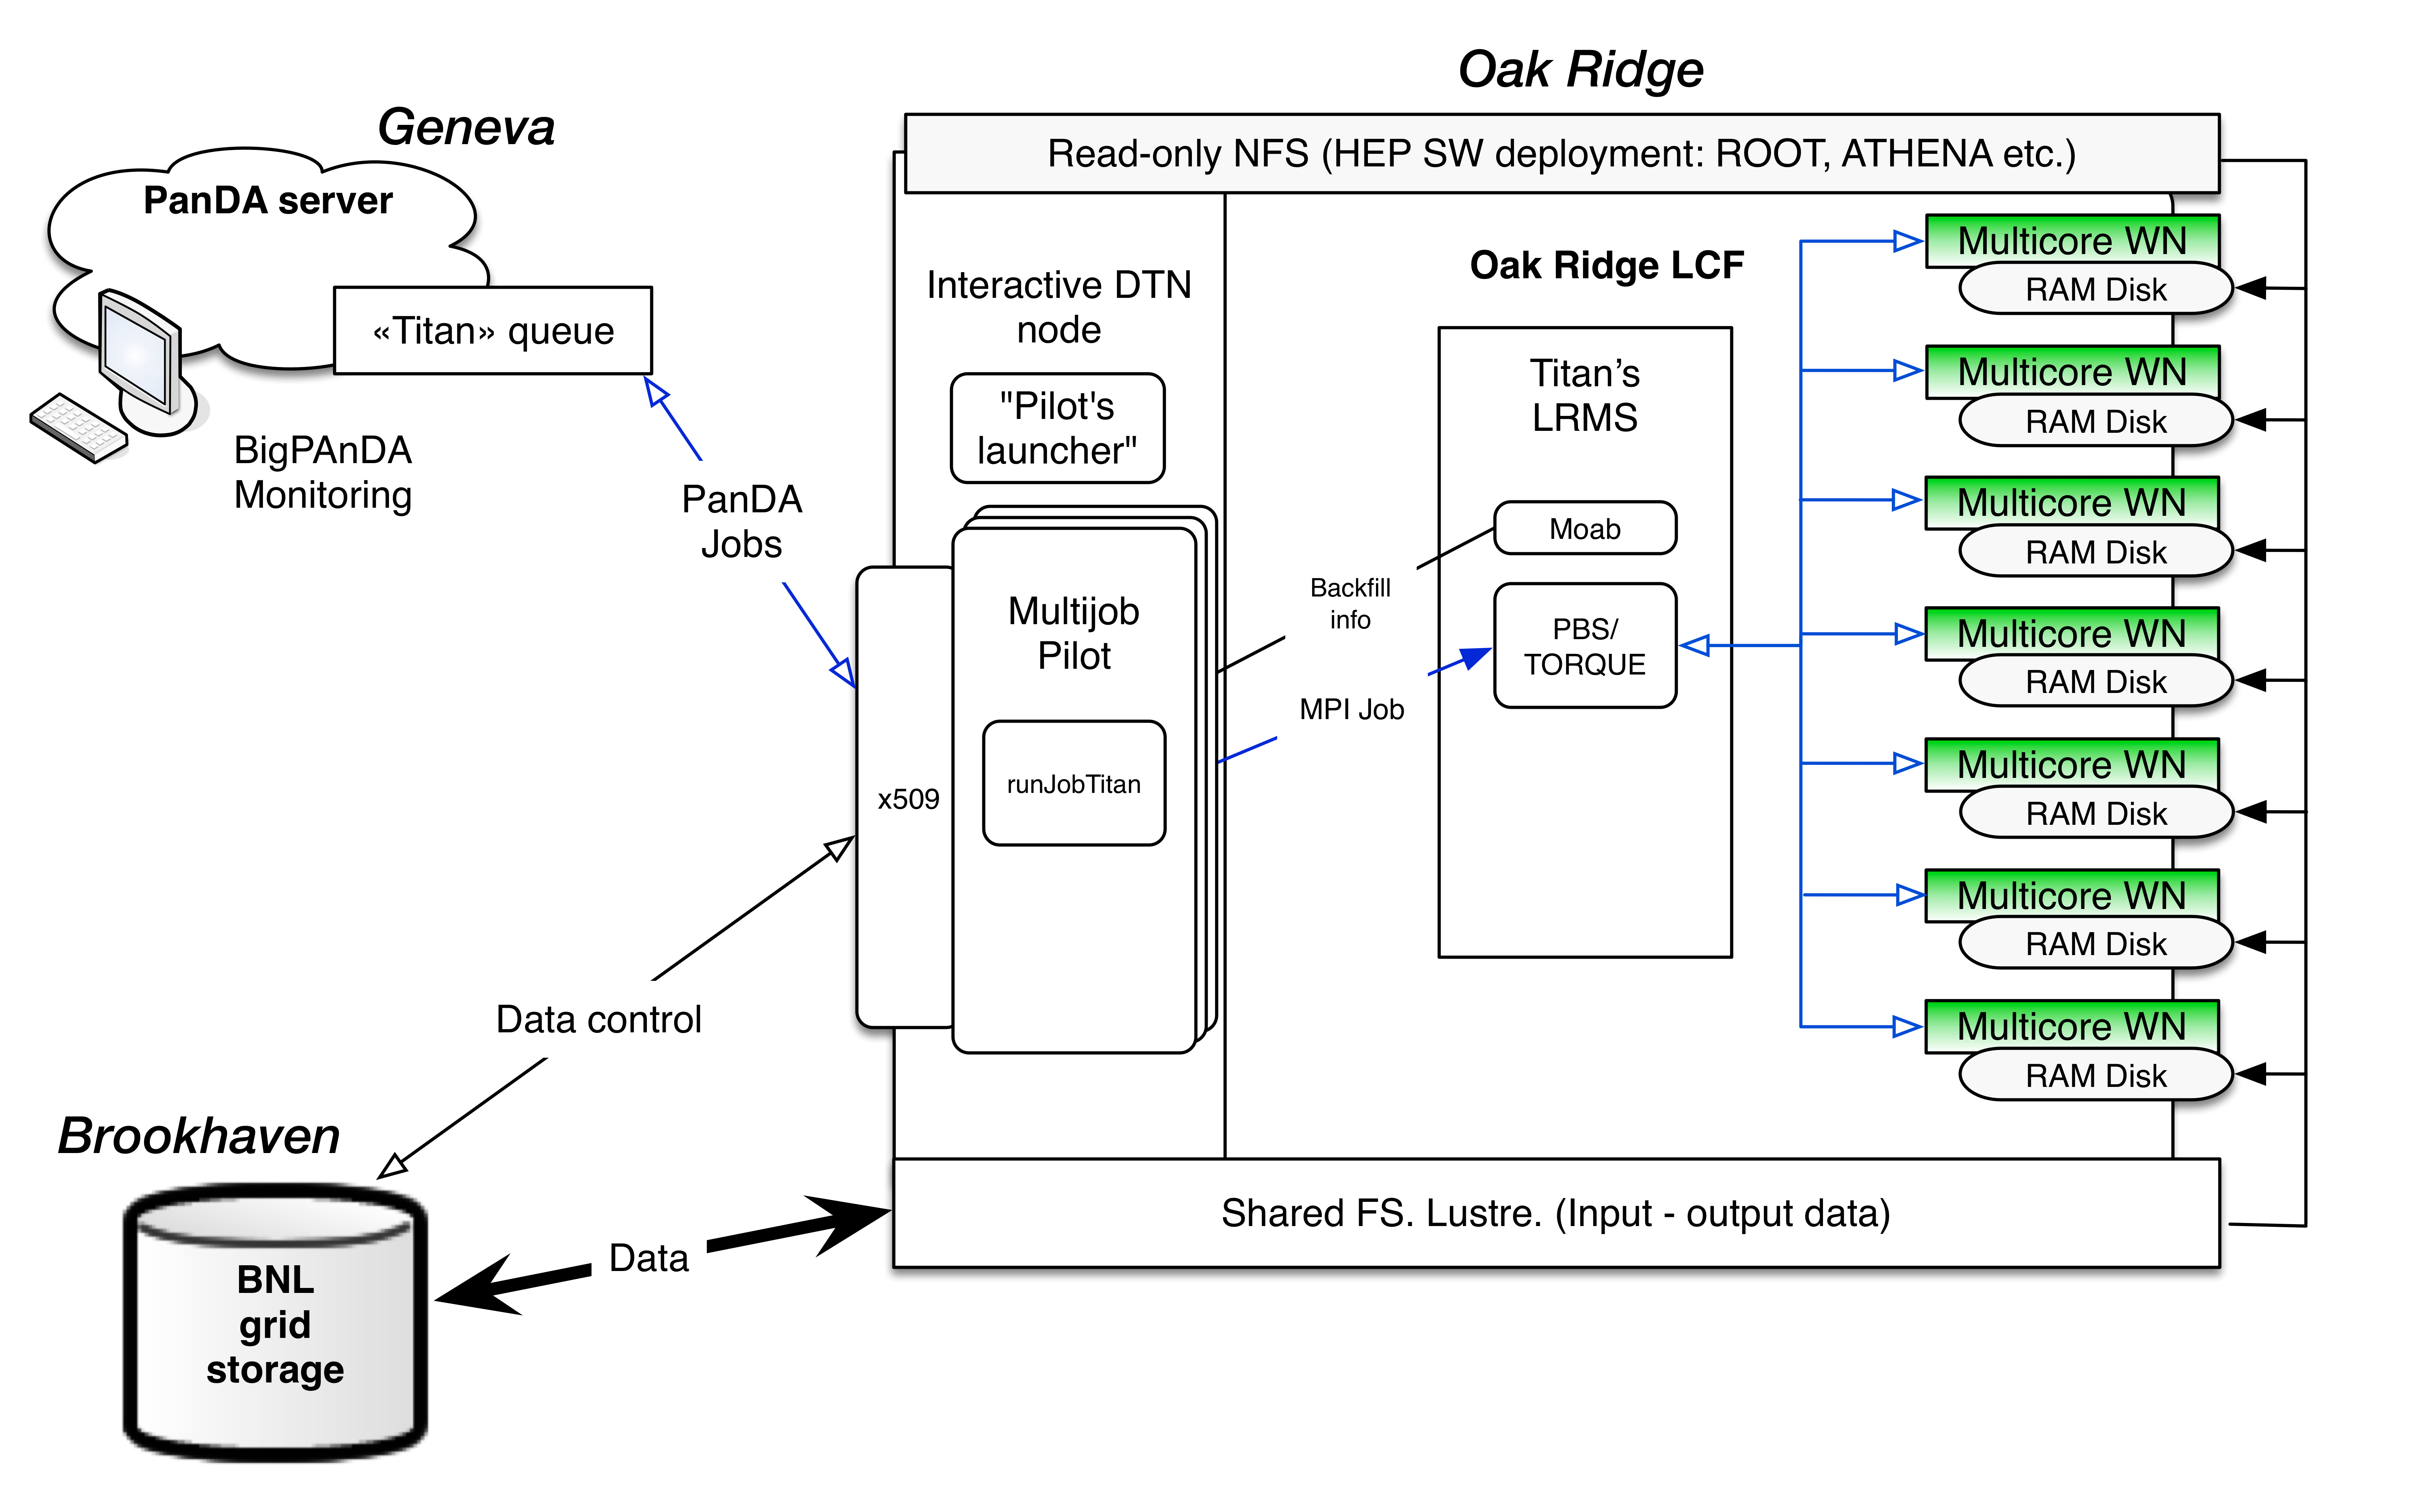
\includegraphics[width=0.75\textwidth]{images/Figure_5.png}
% figure caption is below the figure
\caption{Implementation of PanDA integration with OLCF}
\label{fig:implementation}
\end{figure*}

%-  vim:set syntax=tex:


% ---------------------------------------------------------------------------
% IV - Performance Characterization on Titan
% ---------------------------------------------------------------------------

\section{Performance Characterization on Titan}
\label{sec:performance}
%-  LaTeX source file

%-  performance.tex ~~
%
%   This is the fourth section of the paper.
%
%                                                       ~~ (c) SRW, 23 Sep 2018
%                                                   ~~ last updated 23 Sep 2018

\subsection{Profiling of the performance of the end-to-end workflow on Titan}
\label{subsec:profiling}

% For two-column wide figures use
\begin{figure*}
% Use the relevant command to insert your figure file.
% For example, with the graphicx package use
  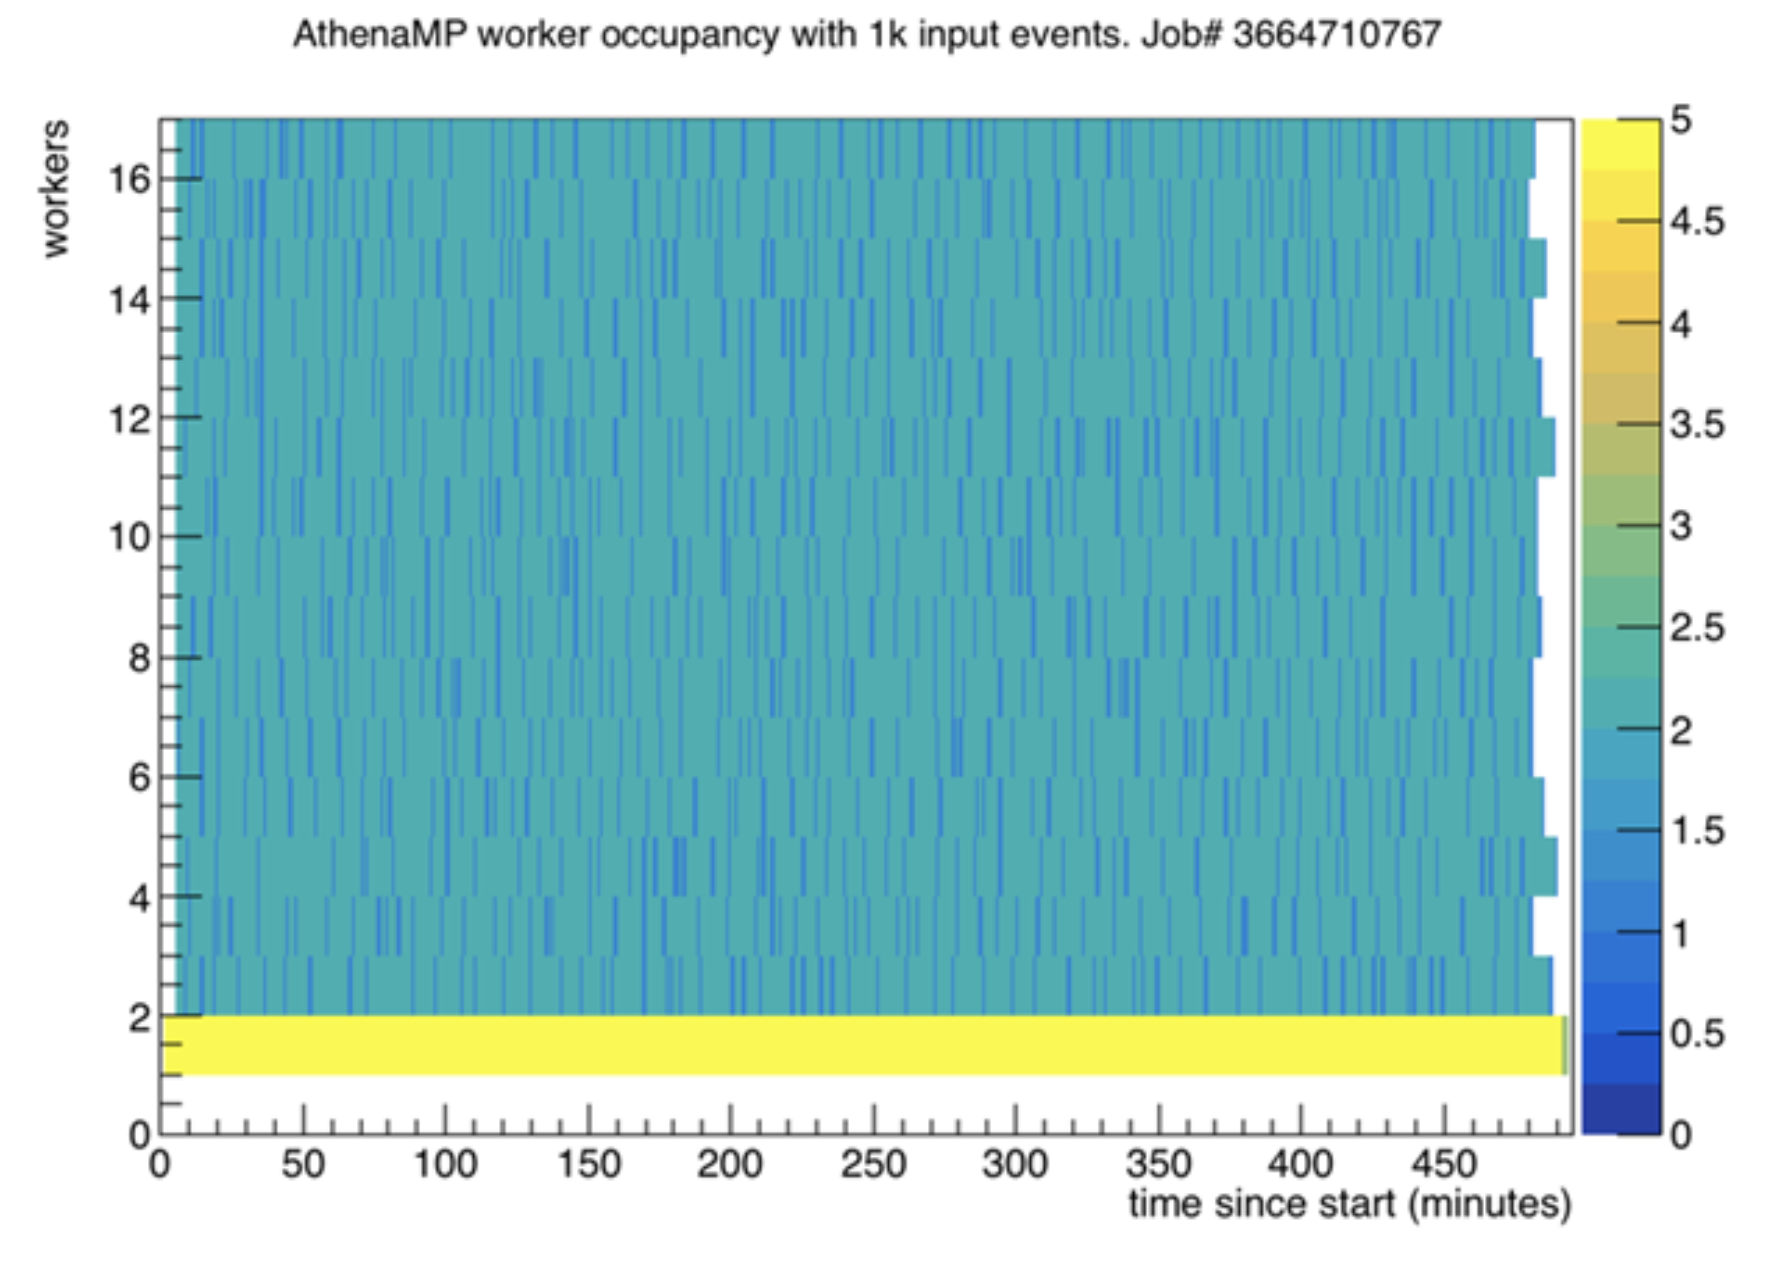
\includegraphics[width=0.75\textwidth]{images/Figure_6_placeholder.png}
% figure caption is below the figure
\caption{AthenaMP worker occupancy for typical ATLAS detector simulation job
with 1000 input events}
\label{fig:athena1000}
\end{figure*}

% For two-column wide figures use
\begin{figure*}
% Use the relevant command to insert your figure file.
% For example, with the graphicx package use
  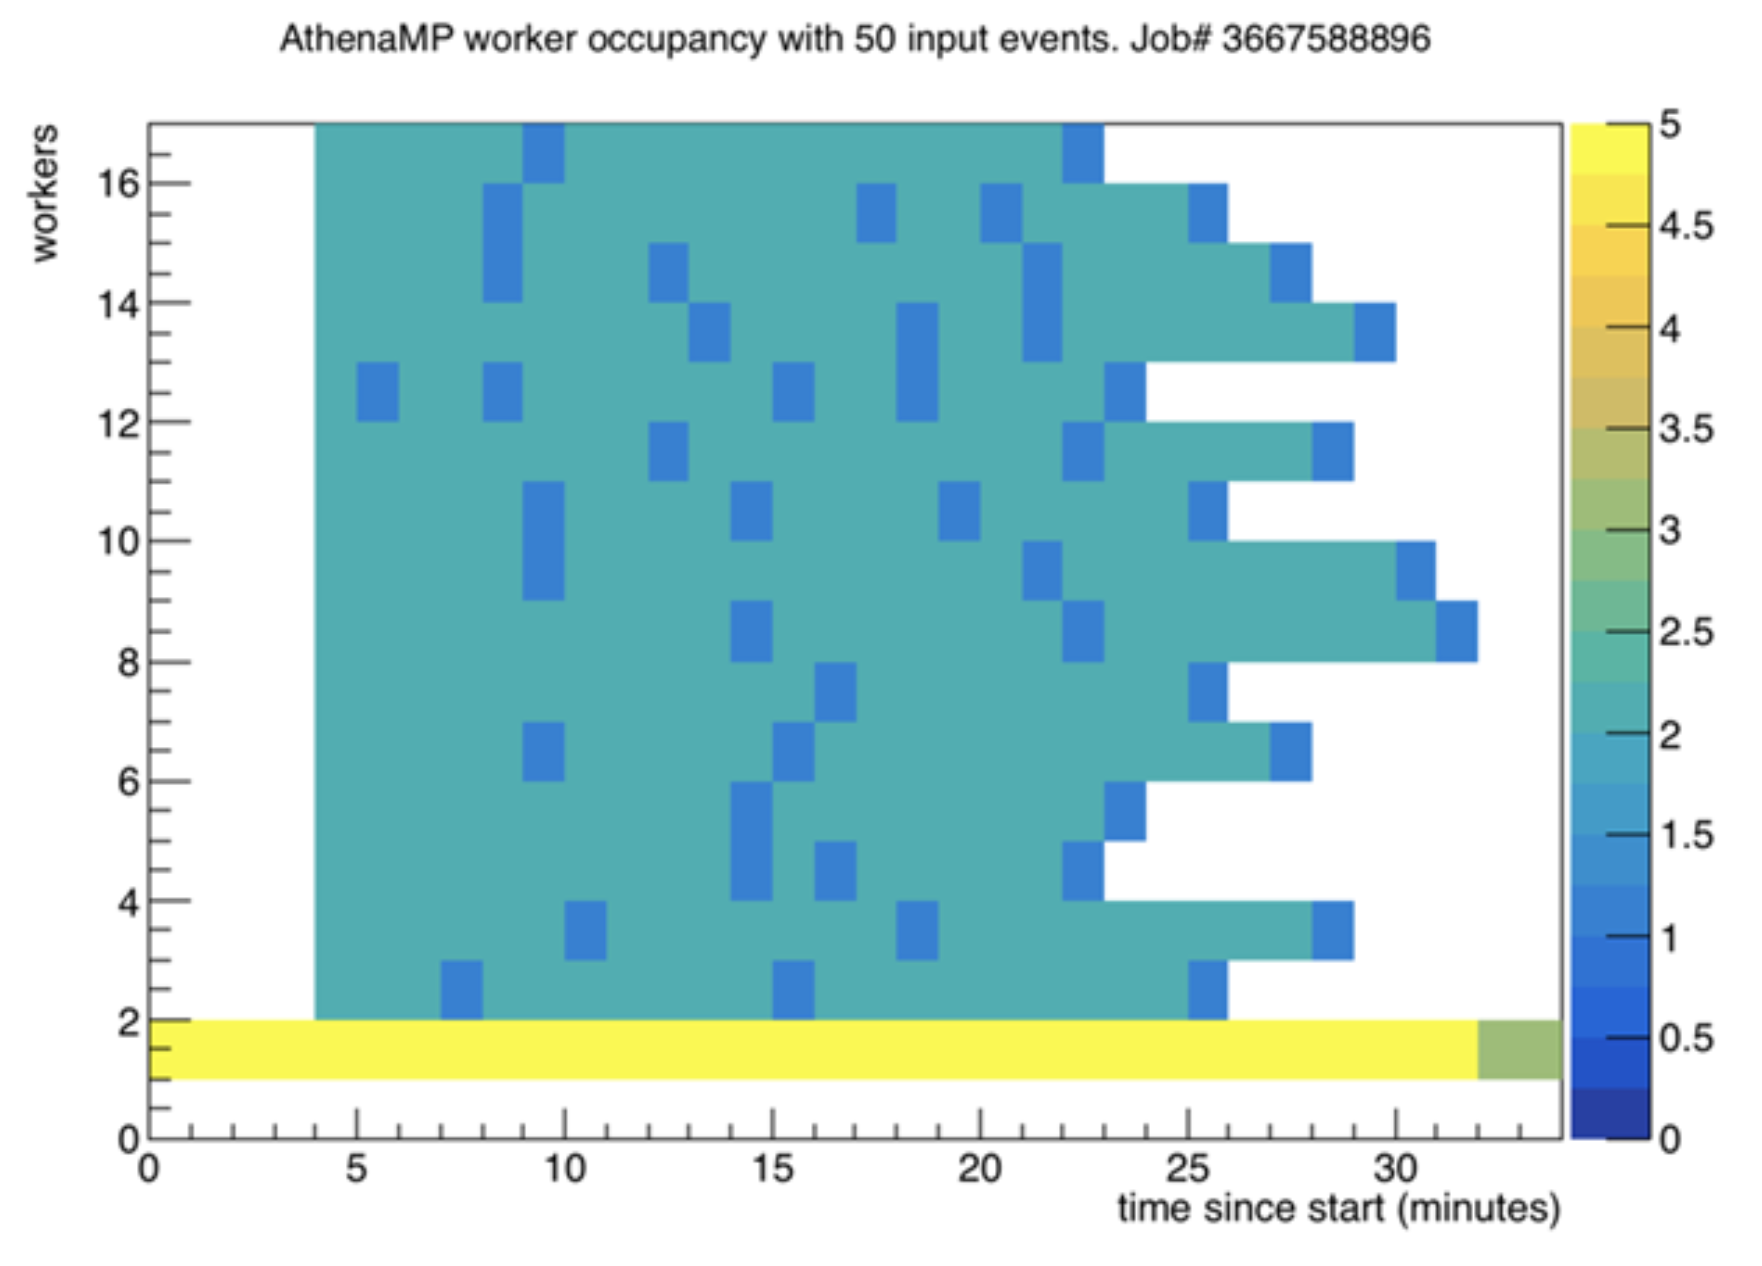
\includegraphics[width=0.75\textwidth]{images/Figure_7_placeholder.png}
% figure caption is below the figure
\caption{AthenaMP worker occupancy for typical ATLAS detector simulation job
with 50 input events.}
\label{fig:athena50}
\end{figure*}

\begin{itemize}
    \item There are two primary objectives:
    \item %
        \begin{enumerate}
            \item some way to characterize the performance (efficiency) of
                PanDa to perform WLMS on LCF (internal), and
            \item some way to characterize the impact of PanDA on Titan
                (external facing).
        \end{enumerate}
    \item Abstract Model of Workload Management System: The common
        functionality that ``all'' distributed workload management systems
        perform, include:
        \begin{itemize}
            \item Manage Payload (i.e., the full set of application workflow)
            \item Get resource information
            \item T2 function of N
            \item Workload Shaping: i.e., decompose Payload into tasks
            \item Job Shaping: i.e., bundle tasks into jobs of defined
                configuration on a resource
            \item Execution management i.e., submit/launch jobs and ensure
                completeness
            \item Data and metadata management, i.e., update central POP with
                job state information.
        \end{itemize}
\end{itemize}

Trying to derive the TTC using the above abstract model of D-WLMS should be our
goal, not a fine grain description of time taken.

These are categories of functionality, not necessarily states. Not all
categories will be exclusive (i.e., unlike states of a job). 

Suggest as a possible consideration to consider the production stream

\subsection{Impact of ATLAS CSC108 on Titan}
\label{subsec:csc108}

The CSC108 project operates under the assumption that the constraints imposed
on its jobs by OLCF prevent it from competing for resources with other
projects. In order to assess the effectiveness of this strategy, we have
pursued several lines of inquiry by sampling data from the MOAB scheduler on
Titan.

Note that code supporting this section is available at
\url{https://github.com/ATLAS-Titan/moab-data}. 

\subsubsection{Blocking Probability}
\label{subsubsec:blockingprobability}

We begin with a simple model that defines an event called a ``block'' and then
detects its occurrences within the data.

Let $C_i$ be the abstract resources in use by CSC108 at the $i^{\text{th}}$
sample point in time, and let $U_i$ be the unused (idle) resources remaining on
Titan. We then define a boolean $B_i$ representing a ``block'' to be 1 if there
exists at least one job at the $i^{\text{th}}$ sample point which requests
$(C_i + U_i)$ resources or less, and we define $B_i$ to be zero otherwise.

Summing $B_i$ over all $i$ gives a count of sample points at which a block
occurred, and dividing that count by the number of total sample points yields a
quantity we will term a ``blocking fraction''.

To use this model for our concrete data set, we define the resources in
question to be requested processors (or requested nodes).

(Specific numbers and graphs go here.)

%-  vim:set syntax=tex:


% ---------------------------------------------------------------------------
% V - Workload Management Beyond HEP
% ---------------------------------------------------------------------------

\section{Workload Management Beyond HEP}
\label{sec:beyond_hep}
%-  LaTeX source file

%-  beyond_hep.tex ~~
%
%   This contains what was originally the seventh section of the Google Docs
%   draft of the paper.
%
%                                                   ~~ last updated 24 Sep 2018

The objective of each subsection is to:
(i) describe the science; and
(ii) detail what customizations had to be done -- either on PanDA or the Titan
    end to support the science driver.
We will then conclude this section with a summary.

\subsection{PanDA WMS beyond HEP}
\label{subsec:panda_beyond}

Traditionally computing in physics experiments at the basic level is usually
independent processing of the input files to produce the output. This
processing in referring in the paper as a job. Processing algorithm usually
utilizes some experiment-specific software which may require parameterization
and even additional configuration files. In the case if such a configuration
file is specific for each job it can be defined in a job as another input file.
Also experiment software may produce some additional files along with the
primary output and they need to be stored. For instance PanDA pilot itself
produces the tar-archive file containing the logs its own logs and the
experiments software logs. Processing algorithm (referenced as ``transformation
script'') responsible for the correct launching the experiment software and
provide all necessary input information including the configuration and run
parameters. PanDA job definition is only defines the launching command for the
transformation script. This launching command is referring as a payload.

The following components are usually provided and controlled by the experiment groups outside from PanDA core components.
\begin{itemize}
    \item Transformation scripts. User groups should define a complete set of
        the transformations scripts to cover all possible SW usage. In the case
        if the same software is used and only the run parameters, configuration
        and input/output file names are changing, the single transformation
        script should be able to cope this.
    \item Input/output files conventions. The size of the input files often
        adjusted in a way to balance of the total processing walltime and
        flexibility in order to cope the failure risks. There is often case
        that the equal sized input files are required relatively equal
        processing time and produce equal sized output. Also input files are
        often named conventionally and grouped in the datasets by some
        attributes. PanDA job definition allows to provide name for the
        input/output datasets.
\end{itemize}

The real workflow for each scientific group provides a lot of additional
requirements and constraints. A common example is a specific order of the jobs
execution. Also implementation of the dedicated workflows demands an
integration with existing experiment computing infrastructure or even
development an additional components. This includes the issues with data
management, user authentication, monitoring, workflow control and etc.

PanDA system may be the best solution for the new experiments and scientific groups by diversity of provided advantages. The main motivations for users are:
\begin{itemize}
    \item Powerful workload management. Automation of the jobs handling,
        monitoring and logging.
    \item Streamlining the usage of the computing resources. Possibility for
        users to run their jobs on diversity of the computing resources. Local
        resource schedulers, and policies are transparent for the users.
    \item PanDA native data handling. PanDA provides a diverse set of the
        plugins to support data stage-in/-out from the remote storages and
        different data movement tools of different types.
    \item Close integration with OLCF. Being integrated with OLCF PanDA system
        also became attractive for many scientific groups already utilizing
        OLCF resources or those who wish to get use them. 
\end{itemize}

Currently, there are few PanDA instances in use by different experiments and groups. 
In this paper, we have considered three instances. The original instance is installed at CERN, 
and it is used exclusively for the ATLAS experiment. Another instance is installed at OLCF, 
and it is dedicated to supporting projects on Titan, subject to OLCF policies. 
Finally, an instance on Amazon’s EC2 cloud infrastructure provides access to multiple independent 
experiments from different disciplines, and it has the least restrictive security and usage policies.

\subsection{PanDA instance at OLCF}
\label{subsec:panda_instance}

In March 2017, we implemented a new PanDA server instance within OLCF operating
under Red Hat OpenShift Origin [Red Hat OpenShift Origin] - a powerful
container cluster management and orchestration system in order to serve various
experiments at Titan supercomputer. By running on-premise Red Hat OpenShift
built on Kubernetes [Kubernetes], the OLCF provides a container orchestration
service that allows users to schedule and run their HPC middleware service
containers while maintaining a high level of support for many diverse service
workloads. The containers have direct access to all OLCF shared resources such
as parallel filesystems and batch schedulers. With this PanDA instance, we
implemented a set of demonstrations serving diverse scientific workflows
including physics, biology studies of the genes and human brain, and molecular
dynamics studies:
\begin{itemize}
    \item Biology / Genomics. 
In collaboration with Center for Bioenergy Innovation at ORNL the PanDA based
workflow for epistasis researches was established. Epistasis is the phenomenon
where the effect of one gene is dependent on the presence of one or more
``modifier genes'', i.e. the genetic background. GBOOST application [GBOOST], a
GPU-based tool for detecting gene-gene interactions in genome-wide case control
studies, was used for initial tests.
    \item Molecular Dynamics.
In collaboration with Chemistry and Biochemistry department of the University
of Texas Arlington we implemented test to try out PanDA to support the
Molecular Dynamics study ``Simulating Enzyme Catalysis, Conformational Change,
and Ligand Binding/Release''. The CHARMM (Chemistry at HARvard Macromolecular
Mechanics) [CHARMM] a molecular simulation program was chosen as a basic
payload tool. CHARMM design for hybrid MPI/OpenMP/GPU computing.
    \item IceCube. 
Together with  experts from the IceCube experiment we implemented the
demonstrator PanDA system. IceCube [IceCube] is a particle detector at the
South Pole that records the interactions of a nearly massless subatomic
particle called the neutrino. Demonstrator includes the use of NuGen package (a
modified version of ANIS [ANIS] that works with IceCube software) - GPU
application for atmospheric neutrinos are simulations packed in singularity
container and remote stage-in/-out the data from GridFTP [GridFTP] storage with
GSI authentication. 
    \item BlueBrain.
In 2017, a R\&D project was started between BigPanDA and the Blue Brain Project
(BBP) [BBP] of the Ecole Polytechnique Federal de Lausanne (EPFL) located in
Lausanne, Switzerland. This proof of concept project is aimed at demonstrating
the efficient application of the BigPanDA system to support the complex
scientific workflow of the BBP which relies on using a mix of desktop, cluster
and supercomputers to reconstruct and simulate accurate models of brain tissue.
In the first phase of this joint project we supported the execution of BBP
software on a variety of distributed computing systems powered by BigPanDA. The
targeted systems for demonstration included: Intel x86-NVIDIA GPU based BBP
clusters located in Geneva (47 TFlops) and Lugano (81 TFlops), BBP IBM
BlueGene/Q supercomputer [BlueGene](0.78 PFLops and 65 TB of DRAM memory)
located in Lugano, the Titan Supercomputer with peak theoretical performance 27
PFlops operated by the Oak Ridge Leadership Computing Facility (OLCF), and
Cloud based resources such as Amazon Cloud.
    \item LSST.
A goal of LSST (Large Synoptic Survey Telescope) project is to conduct a
10-year survey of the sky that is expected to deliver 200 petabytes of data
after it begins full science operations in 2022. The project  will address some
of the most pressing questions about the structure and evolution of the
universe and the objects in it. It will require a large amount of simulations,
which model the atmosphere, optics and camera to understand the collected data.
For running LSST simulations with the PanDA WMS we have established a
distributed testbed infrastructure that employs the resources of several sites
on GridPP [GridPP] and Open Science Grid (OSG) [OSG] as well as the Titan
supercomputer at ORNL. In order to submit jobs to these sites we have used a
PanDA server instance deployed on the Amazon AWS Cloud.
    \item LQCD.
Lattice QCD (LQCD) [LQCD] is a well-established non-perturbative approach to
solving the quantum chromodynamics theory of quarks and gluons. Current LQCD
payloads can be characterized as massively parallel, occupying thousands of
nodes on leadership-class supercomputers. It is understood that future LQCD
calculations will require exascale computing capacities and workload management
system in order to manage them efficiently.
    \item nEDM.
Precision measurements of the properties of the neutron present an opportunity
to search for violations of fundamental symmetries and to make critical tests
of the validity of the Standard Model of electroweak interactions. These
experiments have been pursued [neutron] with great energy and interest since
the discovery of neutron in 1932. The goal of the nEDM [nEDM] experiment at the
Fundamental Neutron Physics Beamline at the Spallation Neutron Source (Oak
Ridge National Laboratory) is to further improve the precision of this
measurement by another factor of 100.
\end{itemize}

To isolate the workflows of different groups and experiments, dedicated queues
were defined at the PanDA server. Presumably in  next steps we will provide the
security mechanisms that will provide the access to each queue for job
submission and dispatching only for authorised users. Also, the PanDA server
provides the tools to customise environment variables, system settings and
workflow algorithms for different user groups. Also this split of the different
groups workflows on the level of PanDA queues simplifies jobs monitoring via
the web based PanDA tool. 

In collaboration with the dedicated scientific groups representatives, we
implemented the ``transformation'' scripts containing complete definition of
the processing actions (set of specific software and general system commands)
are has to be applied to the input data to produce the output. The
transformation script then can be addressed by its name. Client tool provided
to the users allows to submit jobs to the PanDA server with authentication
based on grid certificates. 

Responsible group representative also authorized to run pilots launcher daemon.
Daemon launches the pilots. Number of parallel running pilots can be
configured. Pilots are running and interacts with the PBS under user account
and with Titan group privileges of the responsible representative.

The most important parameters of conducted tests are presented in the table

% For tables use
\begin{table}
% table caption is above the table
\caption{Please write your table caption here}
\label{tab:1}       % Give a unique label
% For LaTeX tables use
\begin{tabular}{llrrrrr}
\hline\noalign{\smallskip}
% ORIGINAL COLUMN TITLES:
%Experiment & Payload/SW & Number of jobs per campaign & Number of nodes per
%job & Walltime (min) & Input data size per job & Output data size per job \\
Experiment & Payload & Jobs & Nodes & Walltime & Input data & Output data \\
\noalign{\smallskip}\hline\noalign{\smallskip}
Genomics           & GBOOST & 10    & 2    & 30 min    & 100 MB & 300 MB \\
Molecular Dynamics & CHARMM & 10    & 124  & 30-90 min & 10 KB  & 2-6 GB \\
IceCube            & NuGen  & 4500K & 1    & 120 min   & 500 KB & 10KB - 4GB \\
LSST/DESC          & Phosim & 20    & 2    & 600 min   & 700 MB & 70 MB \\
LQCD               & QDP++  & 10    & 8000 & 700 min   & 40 GB  & 150 MB \\
nEDM               & GEANT  & 10    & 200  & 20 min    & 120 MB & 20 MB \\
\noalign{\smallskip}\hline
\end{tabular}
\end{table}


\subsection{Summary}
\label{subsec:summary}

The overview of the successfully implemented demonstrations of diverse
workflows implementation via PanDA shows that PanDA model can cope the
challenges of the different experiments and user groups and also provide
possibility for extensions beyond the core components set.  The proof of
concept was received from all considered experiments representatives and
results that PanDA is considered as a possible solution. Preproduction
utilization of PanDA is now under investigation with BlueBrain, IceCube, LSST,
nEDM experiments, LQCD uses PanDA for Production.

%-  vim:set syntax=tex:


%%%

%\section{Section title}
%\label{sec:1}
%Text with citations \cite{RefB} and \cite{RefJ}.
%\subsection{Subsection title}
%\label{sec:2}
%as required. Don't forget to give each section
%and subsection a unique label (see Sect.~\ref{sec:1}).
%\paragraph{Paragraph headings} Use paragraph headings as needed.
%\begin{equation}
%a^2+b^2=c^2
%\end{equation}

%% For one-column wide figures use
%\begin{figure}
%% Use the relevant command to insert your figure file.
%% For example, with the graphicx package use
%  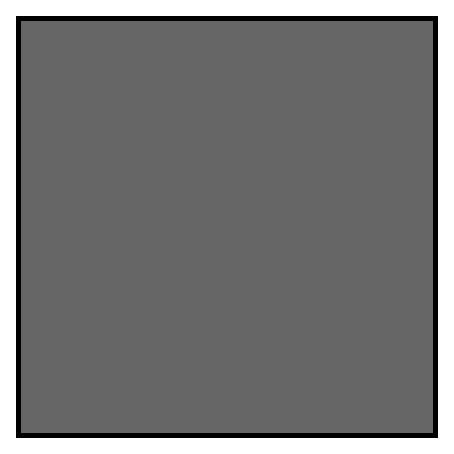
\includegraphics{images/example.eps}
%% figure caption is below the figure
%\caption{Please write your figure caption here}
%\label{fig:1}       % Give a unique label
%\end{figure}
%%
%% For two-column wide figures use
%\begin{figure*}
%% Use the relevant command to insert your figure file.
%% For example, with the graphicx package use
%  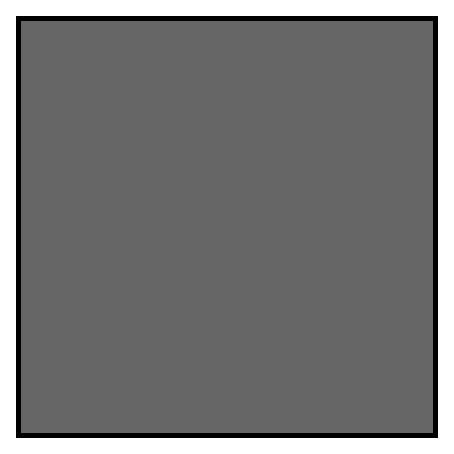
\includegraphics[width=0.75\textwidth]{images/example.eps}
%% figure caption is below the figure
%\caption{Please write your figure caption here}
%\label{fig:2}       % Give a unique label
%\end{figure*}
%%
%
%% For tables use
%\begin{table}
%% table caption is above the table
%\caption{Please write your table caption here}
%\label{tab:1}       % Give a unique label
%% For LaTeX tables use
%\begin{tabular}{lll}
%\hline\noalign{\smallskip}
%first & second & third  \\
%\noalign{\smallskip}\hline\noalign{\smallskip}
%number & number & number \\
%number & number & number \\
%\noalign{\smallskip}\hline
%\end{tabular}
%\end{table}

%\begin{acknowledgements}
%If you'd like to thank anyone, place your comments here
%and remove the percent signs.
%\end{acknowledgements}

% BibTeX users please use one of
%\bibliographystyle{spbasic}      % basic style, author-year citations
%\bibliographystyle{spmpsci}      % mathematics and physical sciences
%\bibliographystyle{spphys}       % APS-like style for physics
%\bibliography{}   % name your BibTeX data base

% Non-BibTeX users please use
\begin{thebibliography}{}
%
% and use \bibitem to create references. Consult the Instructions
% for authors for reference list style.
%
\bibitem{RefJ}
% Format for Journal Reference
Author, Article title, Journal, Volume, page numbers (year)
% Format for books
\bibitem{RefB}
Author, Book title, page numbers. Publisher, place (year)
% etc
\end{thebibliography}

\end{document}
% end of file template.tex

%-  vim:set syntax=tex:
